\documentclass[a4paper,12pt]{article}
\usepackage{geometry}
\usepackage{graphicx}
\usepackage{epsfig}
\usepackage{subfigure}
\usepackage{titlesec}
\usepackage{etoolbox}
\usepackage{xcolor}
\usepackage{listings}

% code format definition
\definecolor{mygray}{rgb}{0.93,0.93,0.93}
\definecolor{mygreen}{rgb}{0,0.6,0}
\definecolor{mymauve}{rgb}{0.58,0,0.5}
\lstset{ %
	backgroundcolor=\color{mygray},
	showspaces=false,
	showstringspaces=false,
	language=Java,
	numbers=left,
	commentstyle=\color{mygreen},
	keywordstyle=\color{blue},
	morekeywords={open,run,imageCalculator,getStatistics,roiManager,setSlice},
	stringstyle=\color{mymauve},
	breaklines=true,
	breakatwhitespace=true,
	columns=fullflexible
	%frame=single
}
% Workarounf of stupid bug: http://tex.stackexchange.com/questions/299969/titlesec-loss-of-section-numbering-with-the-new-update-2016-03-15
\makeatletter
\patchcmd{\ttlh@hang}{\parindent\z@}{\parindent\z@\leavevmode}{}{}
\patchcmd{\ttlh@hang}{\noindent}{}{}{}
\makeatother
% --------------------
\usepackage{marginnote}
% \usepackage[round]{natbib}
\usepackage{url}
\usepackage[colorlinks]{hyperref}
\usepackage{datetime}
\usepackage{hyperref}
\geometry{tmargin=2.5cm,bmargin=3cm,lmargin=1.5cm,rmargin=1.5cm}
\newcommand{\sectionbreak}{\clearpage}

\begin{document}
\title{QuimP Guide}
\author{Piotr Baniukiewicz, Richard Tyson and Till Bretschneider\\ \small Department of Computer Science, Warwick University\\ \small Correspondence to Till Bretschneider. Email: \href{mailto:Till.Bretschneider@warwick.ac.uk}{Till.Bretschneider@warwick.ac.uk}\\}
\date{}
\maketitle
\begin{center}
\textbf{{\large Version: >>>PLACEHOLDER<<<}}\\
\vspace{1cm}
Web site: \url{http://www.warwick.ac.uk/quimp}\\
\vspace{2cm}
This manual is available on GitHub. Feel free to fork it and make pull requests!\\
\url{https://github.com/CellDynamics/QuimP-Doc}\\
\end{center}
\begin{center}
\vfill
{\footnotesize Manual compiled on \today\  at \currenttime}
\end{center}

\tableofcontents

\setlength{\parskip}{10pt}
\setlength{\parindent}{0pt}

\section{License}
The full text of QuimP license is available at \href{https://pilip.lnx.warwick.ac.uk/LICENSE.txt}{https://pilip.lnx.warwick.ac.uk/LICENSE.txt}.

Please, make the following citation in any publication related to our software:

"QuimP [1] used in this study was developed at the University of Warwick with support from BBSRC (BBR grant BB/M01150X/1).”
\begin{enumerate}
\item Piotr Baniukiewicz, Sharon Collier, Till Bretschneider \href{https://academic.oup.com/bioinformatics/article/34/15/2695/4939330}{QuimP: analyzing transmembrane signalling in highly deformable cells}. \textit{Bioinformatics}, Volume 34, Issue 15, 1 August 2018, Pages 2695-2697, \href{https://doi.org/10.1093/bioinformatics/bty169}{doi: 10.1093/bioinformatics/bty169}
\end{enumerate}

\section{PDFs and online versions of this manual}
The user manual exists in two versions, \textit{final} and \textit{development}. The final documentation is (usually) related to the current official release of QuimP, whereas the development version evolves together with the software, following upcoming features, bugfixes, etc.

The most recent documentation can be downloaded from:
\begin{enumerate}
	\item \textbf{Final documentation}
	\begin{itemize}
		\item PDF - \url{https://pilip.lnx.warwick.ac.uk/docs/master/QuimP_Guide.pdf}
		\item HTML - \url{https://pilip.lnx.warwick.ac.uk/docs/master/QuimP_Guide.html}
	\end{itemize}
	\item \textbf{Development documentation}
	\begin{itemize}
		\item PDF - \url{https://pilip.lnx.warwick.ac.uk/docs/develop/QuimP_Guide.pdf}
		\item HTML - \url{https://pilip.lnx.warwick.ac.uk/docs/develop/QuimP_Guide.html}
	\end{itemize}
\end{enumerate} 

\section{About QuimP}
	\begin{itemize}
	\item QuimP software for analysing cellular morphodynamics has been developed on and off since 2002, and was first described in
Dormann D, Libotte T, Weijer CJ, Bretschneider T. \href{https://www.ncbi.nlm.nih.gov/pubmed/12112136}{Simultaneous quantification of cell motility and protein-membrane-association using active contours}. Cell Motil Cytoskeleton. 2002 Aug;52(4):221-30. \href{http://dx.doi.org/10.1007/978-3-0348-8043-5_17}{doi: 10.1002/cm.10048}.
	\item Since then it has contributed to about \href{http://www.warwick.ac.uk/quimp/quimp-refs}{more than 80 publications}.
	\item QuimP development is currently funded through \href{http://www.bbsrc.ac.uk/research/grants-search/AwardDetails/?FundingReference=BB/M01150X/1}{BBSRC BBR grant BB/M01150X/1}: 'QuimP software for quantifying cellular morphodynamics' (PI Bretscheider), Jul 2015-Dec 2018, with Piotr Baniukiewicz as main developer.
	\item Current development aims at making QuimP a sustainable resource for the biomedical community. This involves releasing QuimP as open source for academic use, creating a number of web tools for collaborative development and improved interaction with users.
	\end{itemize}

\section{QuimP - what is new}

\subsection{Summary}
The key features of releases:
\begin{enumerate}
	\item \href{https://pilip.lnx.warwick.ac.uk/site/changes-report.html#a18.10.01}{v18.10.01}
	\begin{itemize}
		\item Optimization of Random Walk module for multi-threading execution (\autoref{sec:RWSeg}).
	\end{itemize}
	\item \href{https://pilip.lnx.warwick.ac.uk/site/changes-report.html#a18.02.01}{v18.02.01}
	\begin{itemize}
		\item Enhanced macro support. The whole workflow can be run as macro - see \autoref{sec:walk_macro}
		\item New module for generating Qconf files from segmented images. It can replace BOA if one has already segmented image - see \autoref{sec:Binary_seg} 
	\end{itemize}
	\item \href{https://pilip.lnx.warwick.ac.uk/site/changes-report.html#a18.01.01}{v18.01.01}
	\begin{itemize}
		\item Macro support - see \autoref{sec:macrosupport}
		\item Save BOA state without quitting - see \autoref{sec:BOAPlugin}, \autoref{sec:boaMenu}
		\item Added option in BOA for expanding snakes from cell inside - see \autoref{sec:BOAPlugin}
		\item Significant changes in Random Walk module, e.g. multi object segmentation - see \autoref{sec:RWSeg} 
	\end{itemize}
	\item \href{https://pilip.lnx.warwick.ac.uk/site/changes-report.html#a17.12.02}{v17.12.02}
	\begin{itemize}
		\item Freeze cells - see \autoref{sec:BOAPlugin}, \autoref{sec:boaWorkflow}, \autoref{sec:boaMenu}
		\item Median Snake filter - see \autoref{sec:boaFilters}
		\item Random Walk plugin - relative error setting, see \autoref{sec:RWSeg} 
	\end{itemize}
	\item New QuimP (after QuimP11)
	\begin{itemize}
		\item The ability to save and restore the state of the BOA plugin for cell contour segmentation. Module configuration, plugin settings and current view are saved in the new file format \textit{QCONF}. To maintain backward compatibility, files in the previous format are can be still generated (refer to \autoref{sec:DataFilesExplained}). The \textit{QCONF} file is human readable using the JSON format and contains all data and parameters generated by BOA. This format is also used by other QuimP modules such as ECMM and Q Analysis. 
		\item New image preprocessing plugins:
		\begin{itemize}
			\item DIC image reconstruction
			\item Random Walker segmentation
			\item Protrusion analysis
		\end{itemize}   
		\item The BOA plugin can use binary masks generated outside QuimP to create cell outlines (Snakes).
	\end{itemize}
\end{enumerate}
	
\subsection{Changelog}
A changelog can be found at the QuimP web page at: \url{https://pilip.lnx.warwick.ac.uk/site/changes-report.html}.
Version of QuimP you are running as well as the version history can be viewed directly from the QuimP Bar plugin (\autoref{fig:quimpBar_menu}).
\begin{figure}[ht]
	\centering
	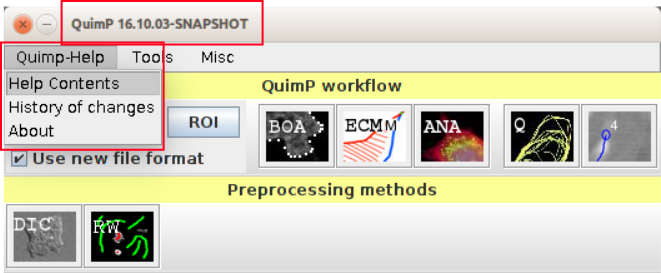
\includegraphics[width=8cm]{quimpBar_menu.png} % requires the graphicx package
	\caption{The QuimP bar}
	\label{fig:quimpBar_menu}
\end{figure}
 	
If you find a bug or have specific feature requests, please contact the QuimP developer:\\ \href{mailto:p.baniukiewicz@warwick.ac.uk}{p.baniukiewicz@warwick.ac.uk}

\section{Installation}

Consult our Wiki page for installation details:\\ \url{http://warwick.ac.uk/quimp/wiki-pages/}

\section{Quick start}
%TODO Keep updated
Matlab routines and walkthrough data mentioned in this section are available from
\href{http://www2.warwick.ac.uk/fac/sci/dcs/people/till_bretschneider/quimp/test_data}{QuimP web page}\footnote{http://www2.warwick.ac.uk/fac/sci/dcs/people/till\_bretschneider/quimp/test\_data}.

Check also our latest publication: \href{https://doi.org/10.1093/bioinformatics/bty169}{Piotr Baniukiewicz, Sharon Collier, Till Bretschneider; QuimP – Analyzing transmembrane signalling in highly deformable cells, \textit{Bioinformatics}}, which contains many examples and workflows in supplementary materials. 

\subsection{Walkthrough analysis, example 1}
\label{walkthrough}

The folder \emph{QuimP\_walkthrough\_files} contains 3 tiff image sequences which you can
analyse (images are courtesy of Evgeny Zatulovskiy, Rob Kay Group, MRC Laboratory of Molecular Biology).

\begin{itemize}
	\item \textit{QW\_channel\_1\_actin.tif}- Actin label.  Image and has been background corrected and contrast enhanced.
	\item \textit{QW\_channel\_2\_neg.tif} - Negative stain.  The cell appears as a shadow on a bright
	background, which has then been inverted.
	\item \textit{QW\_channel\_2\_seg.tif} - For segmentation we shall use the negative stain channel.  
	A 1~pixel Gaussian blur has been applied, the background removed, and contrast enhanced.  
	\item \textit{Segmentation.tif} - Already segmented image - will not be used in this tutorial.
\end{itemize}

\textbf{Step 1}. Open ImageJ and launch the QuimP bar $[Plugins\rightarrow QuimP\rightarrow QuimP Bar]$.  Open the image \textit{QW\_channel\_2\_seg.tif}.  Launch BOA from the QuimP bar.

\textbf{Step 2}. At the prompt check the scale is correct (2 second frame interval, pixel width 0.2 microns).

\textbf{Step 3}. Using the polygon selection tool, create a selection encompassing the cell. This can be very rough.
Click \emph{Add cell}.

\textbf{Step 4}.  Adjust the parameters to get a good segmentation.  Click \emph{SEGMENT} and wait for completion. You can also restore experiment configuration from \textit{QW\_channel\_2\_seg.QCONF} file from \textit{example\_output} folder.

\textbf{Step 5}. Scroll through the sequence to check the segmentation result using either the scroll bar or mouse
wheel. The segmentation should have completed to the last frame.  If not, we will truncate the segmentation.
Scroll to the last frame which successfully segmented and click \emph{Truncate Seg}.
Click \emph{FINISH}, and provide a name for the analysis (e.g. `QTest').

\textbf{Step 6}. Launch the ECMM plugin from the QuimP bar. It does not require an image. When prompted,
locate the QuimP parameter file you just created (e.g QTest.paQP).  ECMM will run.
You can view the result and close the image.

\textbf{Step 7}. Open the image \textit{QW\_channel\_1\_actin.tif}.  With it in focus, launch the ANA plugin,
and again select your parameter file.  Choose a sensible cortex width (e.g. 1.5 microns).
Make sure `save in channel' is set to 1, and normalise to interior is ticked.  Click \emph{ok}.
When complete, ANA will show the sample locations for the last frame.

\textbf{Step 8}. Close \textit{QW\_channel\_1\_actin.tif}, and open \textit{QW\_channel\_2\_neg.tif}.  We will record another
channel for good measure.  Repeat the last step, but with the channel 2 image, this time storing
data in channel 2 (which is the default), and tick \emph{Sample at Ch1 locations}.  ANA will now
use the same sample points as computed for channel 1 (useful if you want to compute ratios between channels).

\textbf{Step 9}. Launch the Q Analysis plugin, and again choose your parameter file. Check your scale is what you expect at the top of the parameter window. We will use all the
current defaults, so click \emph{RUN}.  Inspect your maps, all of which are automatically saved to disk.

\textbf{Step 10}. The displayed images have been scaled to cover the colour space. The raw values have been saved
as text file, with the extension \emph{.maQP} (e.g.  \textit{QTest\_0\_fluoCh1.maQP}).
You can view them in ImageJ by opening them via $[File -> Import -> Text Image...]$. Note that latest versions of QuimP store these files inside \textit{QCONF} configuration file. One can retrieve them by using Format Converter (see \autoref{sec:DataFilesExplained}).

\textbf{Step 11} We will now switch to MATLAB to plot some of this data.  Open Matlab
and open the script file \textit{walkthrough.m}, which will guide you through loading and plotting data.
You can use the output provided in the QuimP package, called \textit{QWalkthrough}, rather than
your own.

You can find the results from above analysis in \textit{example\_output} folder, exemplary post-processing in Matlab are available for viewing  \href{https://pilip.lnx.warwick.ac.uk/docs/Walkthrough.html}{here}\footnote{https://pilip.lnx.warwick.ac.uk/docs/Walkthrough.html}.

\subsection{Walkthrough analysis, macro example}
\label{sec:walk_macro}
In this example you will perform analysis similar to \autoref{walkthrough} but with help of ImageJ macro. Note that this approach requires already segmented image provided as binary or grayscale mask (we use \textit{Segmentation.tif} from walkthrough files). More about converting masks to QuimP format is given in \autoref{sec:Binary_seg}. Below you can find exemplary macro that performs the same anaysis like that described in \autoref{walkthrough}  

\begin{lstlisting}[]
/**
* Exemplary macro running full QuimP analysis.
* 
* Require already segmented image.
* 
* Modify paths before use.
*/

// define where to save main configuration file. It will be shared among QuimP modules.
// Any other file generated by QuimP will be saved in this folder as well
qconfOutput = "experiment.QCONF"
// open segmented image, you can use any other segmentation software to obtain masks
open("Segmentation.tif")
// open original image
open("QW_channel_1_actin.tif")

// 1) perform conversion from mask to QCONF file. This step corresponds to saving segmentation in BOA 
run("Generate Qconf", "opts={options:{" +
	// name of the mask image (nod ID)
	"select_mask:Segmentation.tif," +	
	// name of the image or path here
	"select_original:QW_channel_1_actin.tif," + 
	// density of nodes, step=1 means each pixel of mask will be mapped to node
	"step:4.0,smoothing:true}," +	
	// alternatively path to mask file
	"maskFileName:()," +				
	"paramFile:("+qconfOutput+")}");

// 2) run ECMM analysis on configuration file
run("ECMM Mapping", "opts={paramFile:("+qconfOutput+")}");

// 3) run ANA analysis, we use only one channel
open("QW_channel_1_actin.tif"); // image for intensity sampling
selectWindow("QW_channel_1_actin.tif");
run("ANA", "opts={plotOutlines:true,fluoResultTable:true,fluoResultTableAppend:false," + 
	// configure displaying
	"channel:0, userScale:5.0," + 
	// set channel and cortex width (in um, pixel size from image will be used)
	"normalise:true, sampleAtSame:false," +
	"clearFlu:false," +
	"paramFile:("+qconfOutput+")}");

// 4) run Q analysis
run("QuimP Analysis", "opts={trackColor:Summer," +
"outlinePlot:Speed," +
"sumCov:1.0,avgCov:0.0," +
"mapRes:400," +
"paramFile:("+qconfOutput+")}");

// 5) convert data to csv files	and generate coordinates maps	
run("Format converter", +
	"opts={status:[ecmm:outlines,ecmm:centroid,map:coord,map:origin,map:ycoords,map:xcoords]," +
	"areMultipleFiles:true," +
	"paramFile:("+qconfOutput+")}");
\end{lstlisting}

For latest and actual version of macro check \href{http://www2.warwick.ac.uk/fac/sci/dcs/people/till\_bretschneider/quimp/test\_data}{walkthrough data archive} \footnote{http://www2.warwick.ac.uk/fac/sci/dcs/people/till\_bretschneider/quimp/test\_data}.

\section{QuimP Workflow}

There are four stages which are usually performed when tracking cells using QuimP, each handled by a different plugin (\autoref{fig:quimpBar}).

\begin{enumerate}
	\item Cell segmentation - Performed by the \textbf{BOA} plugin.  Cell outlines, represented as a chain of nodes, are extracted from each frame of an image sequence using an active contour. BOA outputs global measures, such as cell centroid displacement, or cell area.
	\item Membrane tracking - Performed by the \textbf{ECMM Mapping} plugin.  Outlines are mapped between frames to extract local membrane velocities.
	\item Measuring Fluorescence - Performed by the \textbf{ANA} plugin.  Pixel intensities are sampled from the cell's cortex, its width defined by the user.
	\item Data analysis - Performed by the \textbf{Q Analysis} plugin. Statistics are generated and data are visualised in the form of spatial-temporal maps.
\end{enumerate}

Additionally, there are data pre-processing plugins available such as:

\begin{enumerate}
	\item DIC\footnote{Differential Interference Contrast microscopy} plugin (\autoref{sec:DIC})
	\item Random Walker Segmentation plugin (\autoref{sec:RWSeg})
	\item Mask generator (\autoref{sec:MaskGenerator})
	\item Qconf generator (\autoref{sec:Binary_seg})
	\item Format converter (\autoref{sec:ConversionBetweenFormats})
\end{enumerate}

A plugin can be launched from either the $[Plugins\rightarrow QuimP]$ menu, or from the QuimP bar
(opened via $[Plugins\rightarrow QuimP\rightarrow QuimP Bar]$).
Running a plugin will either require an image and/or a QuimP parameter file (with extension \textit{.paQP} or  \textit{.QCONF}) generated by BOA (see \autoref{sec:DataFilesExplained} for details). Demanded file format can be pre-selected by \textit{File Format Selection} tick box. This selection influences all QuimP modules, even if started directly from Fiji plugin menu.
Plugins must be executed left to right, although steps can be repeated without re-running previous plugins and fluorescence measurements performed by ANA can be skipped entirely.

Once complete, data can be analysed in Excel or MATLAB.

\begin{figure}[ht]
   \centering
   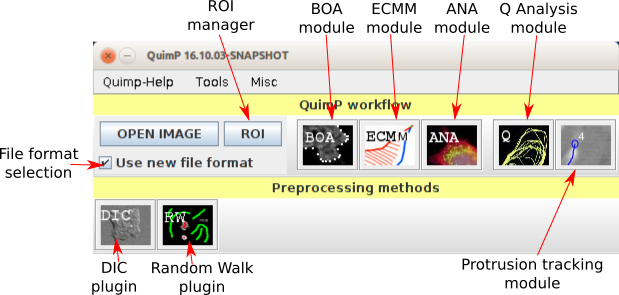
\includegraphics[width=15cm]{quimpBar.png} % requires the graphicx package
   \caption{The QuimP bar}
   \label{fig:quimpBar}
\end{figure}


\section{Cell Segmentation - BOA Plugin}
\label{sec:BOAPlugin}
QuimP utilises an active contour method to segment cells from the background of an image.  Typically, this will be a 
time lapse movie containing a fluorescence channel, captured from a confocal microscope, but the BOA plugin will 
segment any image which has bright objects on a dark background (note that phase contrast images can not be 
segmented with this method).  Attaining the best image for segmentation may require some pre-processing, such 
as the combining of available fluorescence channels (the ideal case is that of an evenly white cell on a black 
background).  \autoref{activeContour} describes the active contour method and provides insight as to BOA's 
parameters.
\\\\
\noindent\fcolorbox{red}{yellow}{
	\parbox{\textwidth} {
		It is expected that objects being segmented have intensity higher than background. Active contour method implemented in BOA will not work for other cases.
	}
}

\begin{figure}[ht]
   \centering
   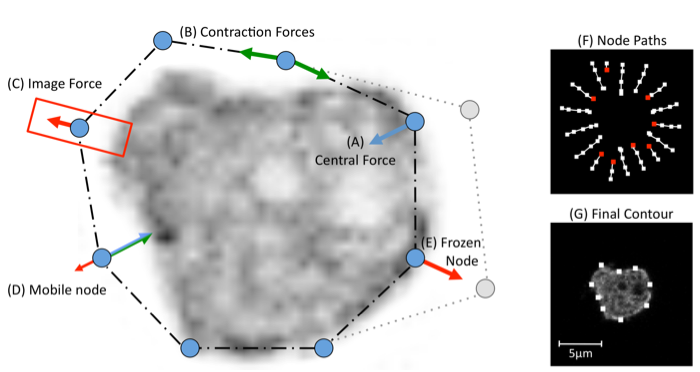
\includegraphics[height=7cm]{activeContour.png} % requires the graphicx package
   \caption{Caricature of outline detection using active
contours.
QuimP's active contour consists of a chain of connected
nodes (a reduced number are shown here for simplicity) initialised
to encircle a cell of interest. Three types of forces act on each
node; (A) Central forces contribute to chain shrinking; (B) Contraction
forces between neighbouring nodes shrink the chain and maintain chain
integrity; (C) Image forces oppose the shrinking of the chain by a
magnitude determined by the local image intensity gradient (red box).
When a node experiences inward forces greater than the opposing
image force it moves inwards (D). On reaching the boundary the image force becomes
sufficiently large to cancel out the other forces, halting and freezing
the node (E). (F) shows the paths of nodes during contraction. Note
that nodes can be added or removed (red nodes) to maintain an average
distance between neighbours. (G) shows the final position of nodes.
QuimP usually makes use of 100 or more nodes to extract high resolution
cell outlines. \cite{Tyson2010}}
   \label{activeContour}
\end{figure}

The BOA window is presented in \autoref{boaWindow}. There are \textbf{four} highlighted areas, which contain tools and allow to adjust settings for segmenting and displaying images, and postprocessing of segmented contours. 
\begin{itemize}
	\item Red: segmentation parameters, described in \hyperref[step4]{step 4} below and buttons:
	\begin{itemize}
		\item \textit{Load} - load \texttt{QCONF} or \textit{paQP} experiment files. The same as \textit{File}$\rightarrow$\textit{Load experiment}, see \autoref{sec:boaMenu}.
		\item \textit{Save} - update loaded experiment. The same as \textit{File}$\rightarrow$\textit{Save experiment}, see \autoref{sec:boaMenu}.
		\item \textit{Copy prev} - copy segmentation settings from previous frame to current one and re-run segmentation for current frame.
		\item \textit{Default} - set default segmentation parameters for current frame..
	\end{itemize}
	\item Blue: controls for navigating through frames in a time series and for zooming cells visible in the current frame. 
	\begin{itemize}
		\item Enabling the tick box labelled \textit{Show paths} will display a trace of the snake as it contracts.  Nodes colour pixels white as they move towards the cell boundary.  This view can be useful for diagnosing why a segmentation fails.
		\item 	Enabling the tick box labelled \textit{Zoom cell}, will zoom the image to selected cell, and track the zoom to the cell's movements.
	\end{itemize}
	\item Green: tools for manual editing of contours.
	\begin{itemize}
		\item \textit{Set Scale} - set pixel size and frame rate. These values can be also read from image file if available or set on the BOA start.
		\item \textit{Truncate seq} - allow to truncate segmented sequence.
		\item \textit{Add cell} - segment current ROI. Segmented cell should be included entirely in ROI. 
		\item \textit{Delete cell} - delete already segmented cell. This option removes the whole track of the cell across frames.
		\item \textit{Freeze} - exclude cell from further modifications. Any changes of segmentation parameters, plugins or segmentation of the whole sequence will not affect frozen cells.
	\end{itemize}
	\item Yellow: access to cell contour postprocessing filters (described in \autoref{sec:boaFilters}). There are also two buttons here helping in populating current filter stack among other frames:
	\begin{itemize}
		\item \textit{Populate fwd} - copy current filter stack (together with configuration of used filters) to all next frames (in contrary to menu \textit{Plugin}$\rightarrow$\textit{Populate to all} that copy current configuration to all frames).
		\item \textit{Copy prev} - copy configuration from previous frame to the current one.
	\end{itemize}
\end{itemize}

\begin{figure}[ht]
	\centering
	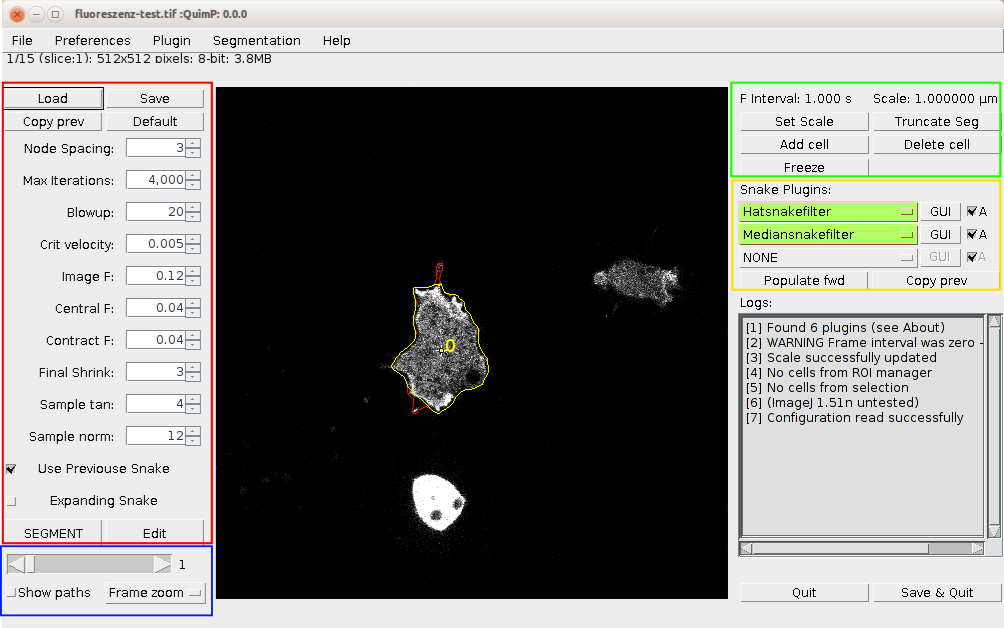
\includegraphics[height=10cm]{boaWindow.png}
	\caption{The BOA Window}
	\label{boaWindow}
\end{figure}

\subsection{BOA menu}
\label{sec:boaMenu}
\begin{itemize}
	\item \textbf{File}
	\begin{itemize}
		\item \textit{Load experiment} - load \texttt{QCONF} configuration file and restore saved state. One can continue work from point where it was saved in. One can load also old \texttt{paQP} files here but program state will not be restored and many configuration options will be missing.
		\item \textit{Save experiment} - update already loaded \texttt{QCONF} configuration file or create new one if such file does not exist.
		\item \textit{Save experiment as..} - save \texttt{QCONF} configuration file under specified name.
		\item \textit{Load plugin preferences} - load configuration of outline plugins stack.  
		\item \textit{Save global preferences} - save configuration of outline plugins stack.
	\end{itemize}
	\item \textbf{Preferences}
	\begin{itemize}
		\item \textit{Plot original} - switch on displaying original outlines together with those processed by plugins. If there is no plugin active (or selected) it does nothing.
		\item \textit{Plot head} - flag zero node of outline with arrow pointing to the outline direction.
		\item \textit{Zoom freezes} - if set, zoom will freeze all cells except that zoomed in. Un-zoom will release all cells.
		\item \textit{Show history} - open history window.
	\end{itemize}
	\item \hyperref[sec:boaFilters]{\textbf{Plugin}}
	\begin{itemize}
		\item \textit{Discard all} - remove all plugins from all frames. Discard all changes introduced by them to the outline.
		\item \textit{Re-apply all} - try to reload plugins from disk and apply them to outlines.
		\item \textit{Populate to all frames} - copy plugin tree from current frame to all other frames and apply it to  outlines. Do not run segmentation. This option can be useful together with \nameref{sec:Binary_seg}.
	\end{itemize}
	\item \textbf{Segmentation}
	\begin{itemize}
		\item \hyperref[sec:Binary_seg]{\textit{Binary segmentation}} - perform binary segmentation on black-white mask 
		\item \textit{Clear all} - remove all segmentation results and set all parameters to their default values
	\end{itemize}
	\item \textbf{Help}
	\begin{itemize}
		\item \textit{Help contents} - open system web browser and try to load this manual. Internet connection is required. 
		\item \textit{About} - display version of QuimP and found plugins
	\end{itemize}
\end{itemize}

\subsection{BOA segmentation workflow}
\label{sec:boaWorkflow}
\textbf{Step 1: Open an image and ensure the correct scale.}  QuimP can segment from a single image, or from an image stack
(but not from a hyperstack).  Only 8-bit images can be used for segmentation and so you will be prompted to convert to 8-bit 
if required.  QuimP uses the scale properties of the image to scale all output to
 microns (pixel size) and seconds (frame interval).  \textbf{ENSURE YOUR SCALES ARE CORRECT} within $[Image\rightarrow Properties...]$.
 On launching, BOA will prompt to check your image scale. The scale is recorded by BOA and stored in the parameter file for
 use in the rest of the analysis. 


\textbf{Step 2: Launch the BOA plugin} 

Unlike previous versions, BOA no longer requires selection of cells prior to launching, but you can do so.  Launch BOA from the QuimP bar or menu.
The BOA window is now a fully functional ImageJ window that allows the user to perform any ImageJ function, such as drawing,
creating ROI's, or zooming while the BOA plugin is in use.  \autoref{boaWindow} shows the BOA window.
The image scale is displayed at the top right.  To adjust the scale click \textit{Set Scale}.      

BOA can segment one, or more cells, each beginning and ending at any frame you wish.  In addition, you can manually 
edit any segmentation at any frame, add/delete cells, truncate segmentations, and adjust the segmentation
parameters for individual frames.

\textbf{Step 3: Adding and deleting cells.} 

To add a cell first scroll to the frame that you want to begin the segmentation at (either with the mouse wheel, or slider).  Using either the
circular, rectangular or polygon selection tool, draw an ROI (region of interest) around a cell, and click \textit{Add cell}. 
BOA will immediately attempt to segment 
the cell at the current frame.  If convergence is successful, the result is displayed as an image overlay. The cell is also given an
identification number.
If the segmentation fails for some reason, the parameters can be adjusted (see below). You do not need to re-add the cell.

Additional cells can be added in the same way.   The active contours surrounding each cell will interact with one another and prevent
contours crossing over to other cells.  This capability is particularly useful in situations where cells come into close contact, 
which often disrupts the segmentation process.

If you are not able to find optimal parameters for many cells at once, you can select only one cell then follow points below and at the end use \textit{Freeze} button to block further modification of this cell. Then repeat the whole process for another cell. Note that \textit{Freeze} freezes the whole sequence and one can has many sequences frozen at one time.   

To delete a cell click \textit{Delete cell}, and then click the centre marker of a cell, on any frame where a segmentation is visible.  Hit the same 
button again to leave delete mode.

\textbf{Step 4: Adjusting segmentation parameters.}.\phantomsection\label{step4}  When a parameter is altered, BOA immediately re-computes the segmentation
for all cells on the current frame with the new parameters (all cells share the same parameters).  Each has a minimum/maximum
value that can not be exceeded.  To alter a parameter either enter a value into the text box, or use the arrows to increase/decrease in steps. The key to attaining a good segmentation is the balancing of the 3 forces.
First, try adjusting the \textit{Image F} parameter to improve the result. Parameters can be set for each frame separately. One can also freeze cell to exclude it from further processing.

The parameters are as follows:

\begin{itemize}
\item \textbf{Node spacing} - Roughly equates to the number of pixels between nodes, and hence the resolution of the segmentation.
\item \textbf{Max iterations} - The maximum number of iterations applied to shrink the contour.
\item \textbf{Blowup} - The number of pixels to expand the solution to the previous frame, for beginning 
calculation at the current frame (utilised when `Use previous snake' is active).  Increase if your target cell is moving by large 
amounts between frames.  Decrease if other cells are coming into close proximity and interfering with the snake.  Lower
values reduce computation time.
\item \textbf{Critical velocity} - The cut-off speed at which nodes are frozen.  Lower the value to allow the snake to continue 
to contract for longer, which may aid in letting nodes enter concavities.
\item \textbf{Image F} - Controls the magnitude of the image force pushing nodes outwards.  This is the most effective parameter 
and should be the first port of call for adjustment.  Highly intense cells will produce high image forces, and you may need to lower 
this value to allow nodes to approach the cell outline.  With weakly intense cells the snake may collapse inwards, past the cell 
boundary, in which case increase the image force.
\item \textbf{Central F} - The magnitude of the central force pulling nodes inwards.  Increase to shrink the snake further and help nodes enter concavities.
Decrease to prevent nodes entering the interior of cells. 
\item \textbf{Contract F} - Magnitude of the force pulling nodes together (i.e. contracting the snake).  Increase to prevent nodes `falling
through holes', or to produce a smoother final solution.
\item \textbf{Final shrink} - The number of pixel to shrink the solution to tighten the snake to the cell boundary.  A value of zero does
not shrink the solution at all.
\item \textbf{Sample tan, Sample norm} - Defines (in pixels) the size of the sampling box around each node within which the 
image is sampled for calculation of the image force.  `tan' describes its width, `norm' its depth.  A larger sampling box will increase 
the size of the image force.  Briefly, the sampling box should be an appropriate size as to give an accurate sample of the local
 intensity between the cell and the background.
\item \textbf{Use previous snake} - If selected, the solution to the previous frame will be used as the starting contour for the current frame.
Otherwise, the users selection is used as the starting contour for every frame.
\item \textbf{Expanding snake} - Experimental option. Rather than contract the snake, it expands it. Initial contour must be drawn inside the cell. Note that all forces are reversed now. 
\end{itemize}

\textit{Buttons and checkboxes:}

Previous segmentation for your image can be loaded
back into BOA by hitting load and selecting a QuimP parameter file with the file extension either \textit{.paQP} or \textit{.QCONF}. Parameter values alone can be loaded by declining to load associated snakes. Button \textit{Default} sets above parameters to their default values and recompute current frame. The \textit{Copy prev} button will copy segmentation parameters from previous frame to the current one and re-run segmentation.

Enabling the tick box labelled \textit{Show paths} will display a trace of the snake as it contracts.  Nodes colour pixels white as they move towards the cell boundary.  This view can be useful for diagnosing why a segmentation fails.


\textbf{Step 5: Segmenting multiple frames.}  When happy with the segmentation on the first frame, hit \textit{SEGMENT} to segment
the cell (or cells) in the following frames. Segmentation parameters from starting frame will be copied to subsequent frames. Any outlines already existing on these frames will be overwritten. The algorithm may fail at a particular frame and a warning will be printed to the log window,
at which point you can alter parameters.plugins. This process can be stopped in any time hitting \textit{SEGMENT} once more.

\textbf{Step 6: Correcting segmentations.}  In the case of failure, or incorrect results, you have 3 options:

\begin{itemize}
\item \textbf{1 - Edit a solution.} Scroll to a frame where an error occurred, click \textit{EDIT} (If you have more than one cell
click its centre). Drag the points of the ROI to the correct locations (you can hold \textit{alt} to delete nodes or \textit{shift to split nodes}).
You can zoom using the imageJ tool (magnifying glass). If you loose your ROI go to $[Edit\rightarrow selection\rightarrow restore selection]$.
Scroll to edit other frames.  When finished, leave edit mode by clicking \textit{*STOP EDIT*}.
\item \textbf{2 - Adjust the parameters.}  Scroll to a frame where an error occurred and change the parameters to improve the segmentation.
Optionally, click \textit{SEGMENT} to apply these new parameters to the following frames.
\item \textbf{3 - Truncate segmentations.}  Scroll to the first frame where an error occurred and click \textit{Truncate Seg'}.  Click the centre
of a cell to remove all segmentations from the current frame onwards.
\item \textbf{4 - Use BOA plugins.} Try to apply available BOA filters for particular frames or for whole stack. Check \textit{Plugin} menu (\autoref{sec:boaMenu}) and \autoref{sec:boaFilters} for details.
\end{itemize}

You can use also \textit{Zoom freezes} feature from \textit{Preferences} to change \textit{Frame Zoom} behaviour. If \textit{Zoom freezes} is ticked on, \textit{Frame Zoom} freezes all already segmented cells except that currently zoomed. Then any modification will apply only to magnified cell. 

\textbf{Step 7: Save the results.}  Click \textit{Save and Quit}.  The saved cell outlines are those visible on the yellow overlay. For new \textit{QCONF} format selected (default) only one composite file is outputted. Otherwise a set of files will be saved for each segmented cell (see \autoref{sec:DataFilesExplained} for description differences between new and old data file format). A cell's ID number is automatically added to filenames.

Enter a name for the analysis (file name extensions are added automatically). BOA outputs files with a \textit{QCONF} extension for new fileformat or \textit{.xxQP} for old one\footnote{QuimP11}.

Files extended  with \textit{.paQP} contain file paths and parameters associated with a particular analysis.  
When running other QuimP plugins, it is the \textit{.paQP} file which you must select to continue an analysis (see \autoref{paQP}).

Files extended \textit{.snQP} contain all data associated with individual nodes of an outline, including pixel coordinates, local cortex 
intensity, local membrane velocities, and tracking data (see \autoref{snQP}).

Files extended \textit{.stQP.csv} contain average statistics per frame, and can be opened directly in 
Excel as a `comma separated file'  (see \autoref{stats}).

The BOA plugin alone outputs many useful statistics regarding cell morphology and migration, without the need to run any further analysis.
Simply open the \textit{.stQP.csv} file in Excel, or use the accompanying scripts to load data into MATLAB (see section \autoref{matlab}).

\subsection{Filtering the outline}
\label{sec:boaFilters}
BOA module supports external plugins for post-processing outlines on current frame. Plugins are standalone \textit{jar} files that can be developed by other scientists and distributed independently from QuimP. Available plugins are discovered when BOA launches by scanning default location, which is Fiji/plugins folder. There is no need of any additional action, discovered plugins are available in filter stack on right (see \autoref{boaWindow}). There are three slots in the stack. Filters are applied in order from most top to bottom, next filter starts with contours returned from the previous one. Any action on filters relates only to current frame (thus each frame can have different filter stack) unless \textit{SEGMENTATION} button is clicked. Automatic segmentation propagates most recent configuration (that means all options available in BOA window) from starting frame to all subsequent frames. Modified contour is drawn in standard yellow colour, whereas red denotes original unprocessed result of segmentation (\autoref{boafilter}). Any further processing in QuimP workflow (e.g. ECMM or ANA) applies to filtered outline. Refer to \autoref{sec:boaMenu} for other options related to filters. \textit{Frozen} cells (\autoref{sec:BOAPlugin}) are also excluded from processing by filters.
\begin{figure}[ht]
	\centering
	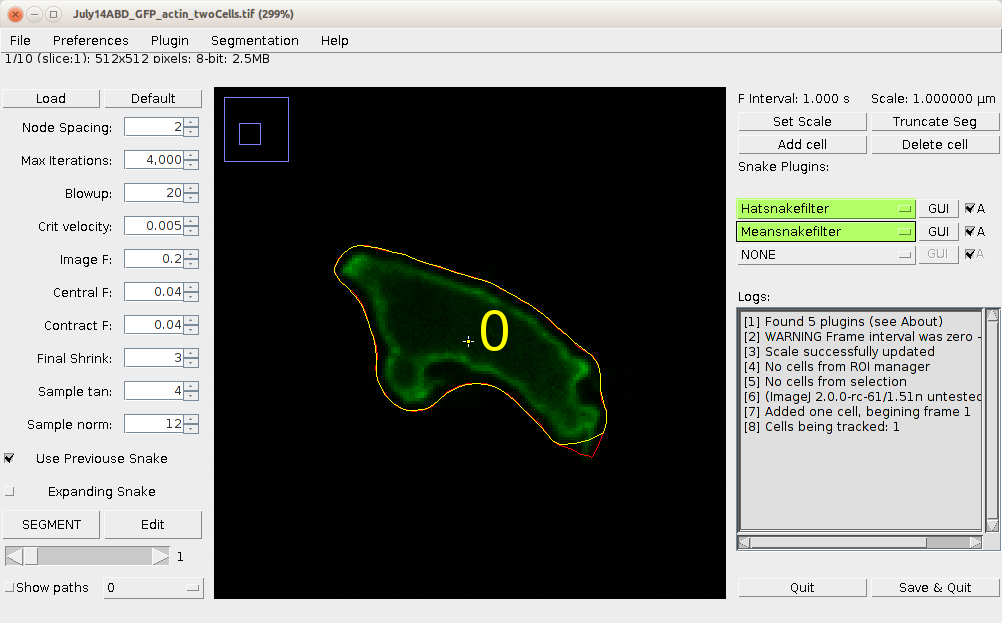
\includegraphics[height=7cm]{boafilter.png} % requires the graphicx package
	\caption{BOA filters in action.}
	\label{boafilter}
\end{figure}

If filter contains an user interface, it can be accessed by \textit{GUI} button (\autoref{boafilter}).

Default installation of QuimP contains four BOA filters:
\begin{itemize}
	\item \textbf{HatSnakeFilter} Removes small protrusions from outlines.
	\item \textbf{MeanSnakeFilter} Apply running mean filter to outlines.
	\item \textbf{MedianSnakeFilter} Apply running median filter to outlines.
	\item \textbf{SetHeadSnakeFilter} Allow to choose first node in snake.
	\item \textbf{RandomWalkSnakeFilter} Perform Random Walk segmentation of frame using Active Contour results (outlines) as initial seed. Refer to \autoref{sec:RWSeg} for more details about Random Walk.
	\item \textbf{HedgeHogSnakeFilter} For testing purposes.
\end{itemize}

Filters that have been discovered and properly loaded are marked in green colour. This is standard behaviour when user start analysis from scratch. If BOA configuration has been restored from \textit{QCONF} file, filters (if any was used) are displayed in red colour to denote that result of segmentation (that is stored in QCONF file together with raw unprocessed outlines) was processed by filter stack but none of those filters is loaded yet to BOA. In this mode user can browse through frames, check segmentation parameters, etc. even if a filter is physically not available in his configuration. Option \textit{Plugin}$\rightarrow$\textit{Re-apply all} will try to load all necessary filters from disk and apply them to each frame where they were used. Note that this operation will recompute all outlines on frames where filters were used and replace loaded results with those evaluated. 

\subsection{A Few Words on Image Segmentation}

If you run into difficulties attaining a good segmentation, there are a few tricks that may help.  If the width of your cell is around 20 pixels or less
try artificially increasing the size of the image with some form of pixel interpolation selected ($[Image \rightarrow Adjust \rightarrow Size]$).
This should aid sampling of the image and allow nodes to enter concavities with greater ease (note, all subsequent analysis
must be performed on the image at the new resolution).

If your images are particular noisy, and cell's appear very grainy, you may try applying a weak Gaussian blur to smooth them
($[Process\rightarrow Filters\rightarrow Gaussian Blur]$).  This should make for more reliable sampling of the cell's interior.

Remember to recalculate the scale of the image when resizing, and to perform intensity analysis on the rescaled image without any interpolation.

Another common approach to improving image quality is to remove background noise using a `blank' image, one taken without any
cells in the field.  This is particularly useful for removing shadows of dirt on the optical equipment, and correcting uneven backgrounds.

\subsection{Binary mask segmentation} \label{sec:Binary_seg}
The QuimP supports creation of Snake outlines directly from binary masks. As the active contour method is not used in this case, one can use another segmentation algorithms (e.g. \hyperref[sec:RWSeg]{Random Walker method}) to deal with problems that typically occur for active contour such as e.g. bad segmentation of cavities.

To use binary segmentation, either black-white mask (8-bit image in ImageJ) or grayscale images should be obtained in any other way, e.g. by using alternative segmentation tools. It has to be size of segmented image that is already loaded to BOA plugin. The number of slices in mask file should be less or equal to the number of slices present in segmented image. \textbf{The background pixels must have value 0 whereas objects can be defined by any other values within the range 1-255}. This plugin is capable to perform simple cell tracking between adjacent frames. If input mask is binary then cells are assigned to the same track by testing their overlapping between frames. For grayscale images, numeric values of pixel intensities are used.

The binary segmentation plugin can be launched from BOA menu $(\textit{Segmentation}\rightarrow \textit{Binary segmentation})$ or as standalone module from QuimP Toolbar. The latter method supports also IJ macros. If one calls this plugin as separate external module from QuimP Toolbar or IJ menu, it will produce Qconf file in the same way as BOA module does. This file can be than passed to other QuimP modules for further analysis.   

\begin{figure}[!h]
	\centering
	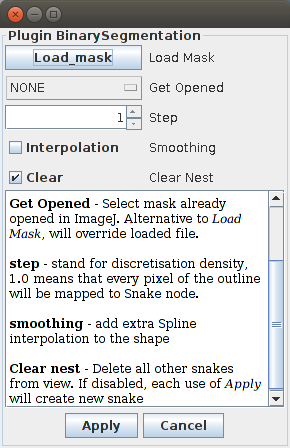
\includegraphics[height=8cm]{BinarySeg.png}
	\caption{The Binary Segmentation Window}
	\label{BinarySegWindow}
\end{figure}

The mask can be either loaded from separate file (ImageJ formats are supported) or selected among already opened images in ImageJ. Results of segmentation are displayed in real-time on BOA window immediately after clicking \textit{Apply}. \textit{Cancel} closes the plugin window leaving last results of segmentation in BOA. If \textit{Clear} is selected each use of \textit{Apply} will clear current outlines in BOA. If it is unselected, outline will be added to BOA. Note that each click on \textit{Apply} will create new outline even if non of plugin parameters is modified. 
Resulting outline can be smoothed by e.g. \texttt{MeanSnakefilter} available in the plugin area (see \autoref{boaWindow}). Filter can be applied for selected frames only or populated for the whole sequence by $(\textit{Plugin}\rightarrow \textit{Populate plugins})$
 
\section{Cell Tracking - ECMM Plugin}

To extract data on local membrane velocity QuimP utilises our Electrostatic Contour Migration Method (ECMM).  
Nodes that form a cell outline at time \textit{t} are mapped onto the segmented outline at time \textit{t+1}.  The distance a node migrates
during the mapping process, and the frame interval, determines the local membrane velocity at the node's position.  If you only have a single
frame there is no need to run this plugin.  ECMM edits and adds to data 
already contained within an \textit{.snQP} file.

\textbf{Step 1: Launch the ECMM Mapping plugin, and open the desired \textit{.paQP} file when prompted.}  There are no parameters that
require manual setting.

\textbf{Step 2: Inspect the results}.  The blue outline represents the cell outline at time $t$, the green at time $t+1$.  
Green circles, overlaid with crosses, denote intersection points that have been validated and used for calculating sectors.  
Red lines denote paths taken by migrated nodes.   Nodes that fail to map correctly are highlighted in yellow.
Failed~node (FN) warnings are displayed along with a running total (in brackets) of the number of failed nodes in the whole sequence.  
The log window will display progress and warnings. 

If a node fails to map it is simply ignored, the effect of this is a small reduction in mapping resolution at the nodes location.
If the process fails to map the majority of the nodes correctly, then a new segmentation will have to be performed
(try using a different node resolution or changing the image resolution).

\subsection{ECMM Tracking}
\label{ecmmTracking}

The details as to the workings of ECMM can be found in our publication \cite{Tyson2010}.
The current implementation includes several significant improvements.  It is not necessary to understand the method,
only the format of the tracking.

At frame $t=1$ a node is randomly chosen as being node zero, $n_{0}$.  Other nodes are then assigned a position
according to their distance from $n_{0}$ along the cell perimeter.  The length of the cell perimeter 
is normalised to $1$, hence the position of a node which is exactly half way around the perimeter will be 0.5
(see \autoref{ecmm}a).

\begin{figure}[ht]
   \centering
   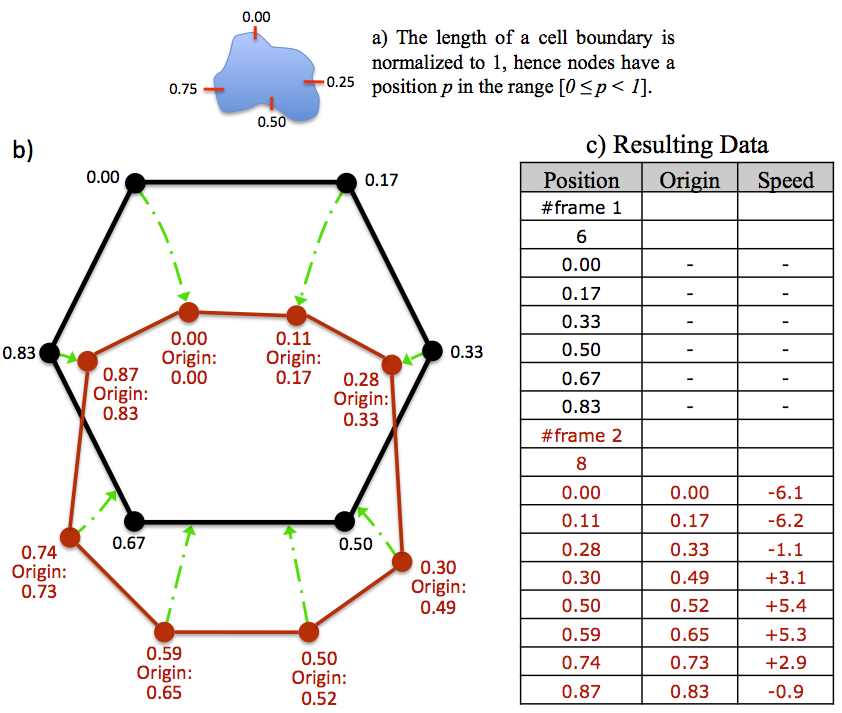
\includegraphics[height=10cm]{ecmm.png}
   \caption{\textbf{ECMM tracking method. a)} Normalisation of the cell perimeter. \textbf{b)} Caricature of the tracking of node positions
   between two frames (black $t$, red $t+1$). Arrows pointing towards the red outline indicate forward mappings and a nodes origin is recorded simply
   as its position on the black outline. Arrows pointing towards the black outline indicate reverse mapping and node origins
   are recorded as interpolated values between nodes on the back outline.
    \textbf{c)} Data from \textit{b)} as it would appear in a \textit{.snQP} file. The frame number is followed by the number of nodes in the outline.
    Speeds are proportional to the lengths of the green mapping arrows.}
   \label{ecmm}
\end{figure}


The nodes of the outline at $t=2$ also have positions assigned, but in addition have an \textit{origin}.  This represents 
where a node originated from on the $t=1$ outline.  For example, a node with an origin of 0.5 originated from 
position 0.5, exactly half way around the outline at $t=1$.

It should be realised that this method of tracking is sub-node resolution.  By simply interpolating the positions and origins of 
nodes, any real number position on an outline can be tracked at sub-node resolution, for as many frames as desired.  See \autoref{snQP} for the format of data output, and \autoref{trackingMaps} for using ECMM data within MATLAB.


\section{Fluorescence Measurements - ANA Plugin}
\label{ana}

QuimP samples the intensity of pixels from within the cortical region of a cell.  At each frame, nodes of the cell outline
are shrunk inwards to form an inner outline.  The amount of shrinkage is specified by the user, and relates to the
estimated cortex width.  Nodes are 
migrated inwards towards the inner outline, while simultaneously measuring pixel intensities  (a 3x3 average).  
A nodes fluorescence intensity is the maximum recorded as it migrates across the cortex.  ANA can record data for up to 3 separate 
fluorescence channels.

\begin{figure}[ht]
   \centering
   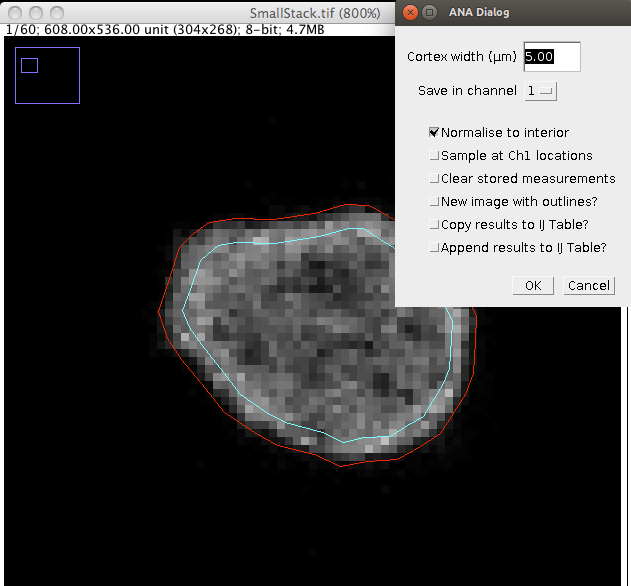
\includegraphics[height=8cm]{ana.png} % requires the graphicx package
   \caption{ANA.  The area between the red and blue contours is the user defined cortex, and is where
   intensity samples are taken. If \emph{Normalise to interior} is ticked, sampled intensities will be normalised
   to the average intensity of pixels within the blue contour.}
   \label{fig:ana}
\end{figure}

\textbf{Step 1: Open an image stack containing the desired fluorescence channel.}  This may be the same stack used 
for cell segmentation, or one containing data from another channel.  Ensure the opened stack has the 
same resolution and number of frames as that used for segmentation.

\textbf{Step 2: Launch the ANA plugin and open the desired \textit{.paQP} or (recommended) \textit{QCONF} file when prompted.}

\textbf{Step 3: Enter a value for the cortex width ($\mu m$) and choose a channel.}  The inner and outer outlines
are displayed on the image.  Changing the cortex width will update the image overlay.
Choose a channel to record data in from the drop down menu.

ANA provides 5 further options
\begin{itemize}
	\item Normalise to interior - Toggle normalisation of intensity sampling to the cells interior (recommended).
	\item Sample at Ch1 locations - Sample at the same locations as determined for channel 1.
	\item Clear stored measurements - Removal all fluorescence measurements from QuimP's files.
	\item New image with outlines? - Produce copy of input image stack with inner and outer outlines in it. Outlines are drawn at overlay\footnote{\url{https://imagej.nih.gov/ij/docs/guide/146-11.html}}. Flatten the image before using it in another software.  
	\item Copy results to IJ table? - Open standard ImageJ table\footnote{Standard table always is named \textit{Results}} filled with fluorescence statistics computed for selected channel (the same are written to\textit{stQP.csv} file). Note that is an experiment contains more than one cell, ANA will be run for each of them separately but finally the table will always contain statistics for all cells. 
	\item Append results to IJ table - works as \textit{Copy results to IJ table?} but does not clear table before. Can be used for collecting results from different experiments. 
\end{itemize}

Click \textit{OK}.
  
Fluorescence data associated with specific nodes is saved in the \textit{QCONF} file and additionally in \textit{.stQP.csv}.

\textbf{Step 4: For further channels, open the next channel image and re-run ANA.}

\section{Compiling Data - Q Analysis Plugin}

Data within \textit{QCONF} file (or \textit{.snQP} and \textit{.stQP} for old path\footnote{Refer to \autoref{sec:DataFilesExplained}}) files can be read into Matlab at this point, but motility maps have not yet been generated\footnote{If old path is selected, otherwise one should use Format Converter tool to obtain these files. Refer to \autoref{sec:DataFilesExplained}}.
The Q Analysis plugin will build spatial-temporal maps of motility, fluorescence, and convexity,
and also several other maps to aid analysis.  In addition, vector graphics are produced 
using the \textit{Scalable Vector Graphics} format.  These include a cell track in which all cell outlines are overlaid and coloured
according to frame number, and a motility movie in which nodes are coloured with a user specified data type.

\textbf{Step 1: Launch the Q Analysis plugin and open the desired \textit{.paQP} file when prompted}.

\begin{figure}[ht]
   \centering
   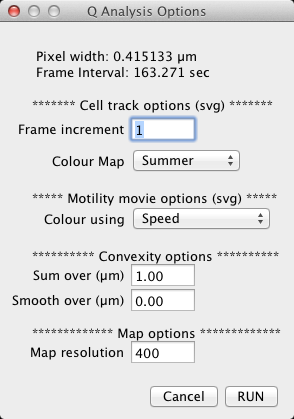
\includegraphics[height=8cm]{screenQAnalysis.png} 
   \caption{Q Analysis options dialog}
   \label{screenQAnalysis}
\end{figure}

\textbf{Step 2: Enter parameters to the options dialog}.  The parameters are as follows:

\begin{itemize}

\item \textbf{Cell track option - Frame increment}  [positive integer].  The frame increment for drawing the
cell track (\textit{\_track.svg}).  Frames are only draw at the specified increment.  Set to 1 for all frames.  
\item \textbf{Cell track option - Colour Map}.  Select a colour scheme for the cell track.
\item \textbf{Motility movie option - Colour using.}. Select the data type for use in colouring nodes of the motility movie.
\item \textbf{Convexity option - Sum over (microns)} [positive real number].  Distance around the cell 
perimeter ($\mu m$) to sum curvature. Set to zero for no summation.
\item \textbf{Convexity option - Smooth over (microns)} [positive real number].  Distance around the cell 
perimeter ($\mu m$) to over which to average curvature for smoothing. Set to zero for no smoothing.
\item \textbf{Map option - Map resolution} [positive integer]. A value of $x$ will produce images that are
$X$ pixels in width.  The height of the image will be equal to the number of frames of the analysed sequence,
or a multiple of number of frames (if less then $x$). Data is interpolated to form maps of any size.
\end{itemize}

The images produced are for visualisation only, as they have been scaled to fill the RGB colour spectrum.
Vertical image scale is set to frames (frame zero at the top),
horizontal to the normalised length of the cell perimeter (0,1].
Import $.maQP$ files as text images for further analysis in ImageJ. See Section \autoref{maps} for details
and analysis of maps.

\section{QuimP preprocessing plugins}
\label{sec:QuimP_preplugins}
\subsection{DIC images processing}
\label{sec:DIC}

Differential interference contrast microscopy (DIC) enhances the contrast in unstained, transparent samples. DIC images can be easily interpreted and analyzed by biologists due to high resolution available and excellent contrast generated by steep gradients in optical path lengths and phase shifts between the two polarized beams. Nevertheless, very characteristic bas-relief observed in DIC images is the source of problems in automatic analysis of these images. The image contrast and the same the object’s boundaries are well defined in the shear angle but in direction perpendicular to it there is no contrast against to background and thus a lack of distinct edges of object. Moreover, strong gradient of image intensity at shear angle negatively influence standard image processing methods like global thresholding or edge detection producing insufficient results, with discontinuous regions or edges.

The DIC plugin provided with QuimP allows to convert DIC samples into form more suitable for segmentation and further image processing. The local contract for any cell in reconstructed image is well defined in every direction and the intensities of pixels take only positive values (in relation to a mean intensity level). The algorithm implemented in QuimP is described in \cite{Kam1998}. Either single images or time lapse movies from DIC microscopy can be processed. 

\textbf{Step 1: Open an image.}
Once loaded into ImageJ/Fiji click DIC filter in QuimP bar. Only 8-bits images are supported (256 gray levels).

\textbf{Step 2: Set correct parameters}
There are two important parameters: \textit{Shear} angle and \textit{Decay} (Fig. \autoref{fig:dicdialog}). The \textit{Shear} parameter is the shear angle of DIC microscopy measured counterclockwise, whereas \textit{Decay} is described in details at \cite{Kam1998}. The \textit{Decay} factor depends mainly on the size of cells and the best results are usually achieved experimentally. \textit{Invert output} option inverses colorscale in reconstructed image.

Reconstructed image can be affected by linear pattern that can be filtered by running mean filter activated if \textit{Filter mask size} is greater than 0. Smoothing filter is applied before processing for angle perpendicular to given \textit{Shear}\footnote{Currently, smoothing can be used only with the following shear angles: 0, 45, 90, 135. For another values it will run for closest multiplicity of 45 degrees.}.
   
\begin{figure}[ht]
	\centering
	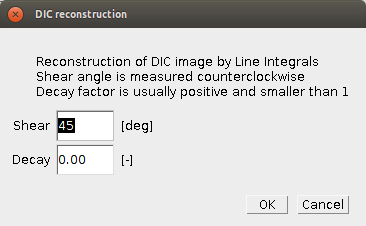
\includegraphics[width=8cm]{DICwindow.png} 
	\caption{DIC filter options dialog}
	\label{fig:dicdialog}
\end{figure} 

\noindent\fcolorbox{red}{yellow}{
	\parbox{\textwidth} {
		If objects (cells) in reconstructed image are darker than background, the image should be inverted before further processing in BOA module. One can use ImageJ option \texttt{Edit$\rightarrow$Invert} or tick \textit{Invert output} in plugin window. Refer to \autoref{sec:BOAPlugin}.
	}
}

\subsection{Random Walker Segmentation}
\label{sec:RWSeg}
The Random Walks Segmentation algorithm is described in the paper \cite{Grady2006}. It belongs to the class of supervised segmentation algorithms what means that the user interaction is needed. In RW method a user has to specify a small set of pixels belonging to the desired object and (possibly) a set of pixels belonging to the background. Those pixels are called \textit{seed pixels} and in this plugin they form the seed image. The seed image must be the size of segmented image whereas, the number of layers can be either equal to number of layers in segmented image or set to 1. 

This plugin supports also multi-object segmentation, where user defines several foreground objects (up to 255). For this case, the output is a grayscale image where each unique object is marked by different colour, starting from 1. 

Segmentation is run in two sweeps. First one gives rough segmentation whereas the second one produces final result. Second sweep uses binary mask produced by the first step as an input after filtering it by selected \textit{Binary filter}. Second sweep can be disabled by setting \textit{Gamma 1} to 0 (disabled by default, use with care as it can give unpredictable results in some cases). By default second sweep uses half of defined iteration number.

For best results, the background seeds should be drawn close to foreground objects. 

Implemented algorithm uses iterative scheme with three possible stopping criteria:
\begin{enumerate}
	\item ITERATIONS - if number of iteration defined in \textit{Iterations} is exceeded for first sweep or half of this number for the second sweep (if enabled).
	\item NANS - if Infs or NaNs appear in solution (they will be removed before outputting result)
	\item RELERR - if relative error is smaller than defined. Defined by \textit{Rel error}.
\end{enumerate}

The RW plugin can be called outside of QuimP from the QuimP Bar, from IJ macro or directly from API. The main interface is presented in \autoref{fig:rwdialog}. The window is divided into eight sections:
\begin{enumerate}
	\item Image section
	\item Seeds section
	\item Dynamic section that depends on selection in previous section
	\item Segmentation options section
	\item Inter-processing section
	\item Local mean feature section
	\item Post-processing section
	\item Display options section
\end{enumerate}

\begin{figure}[ht]
	\centering
	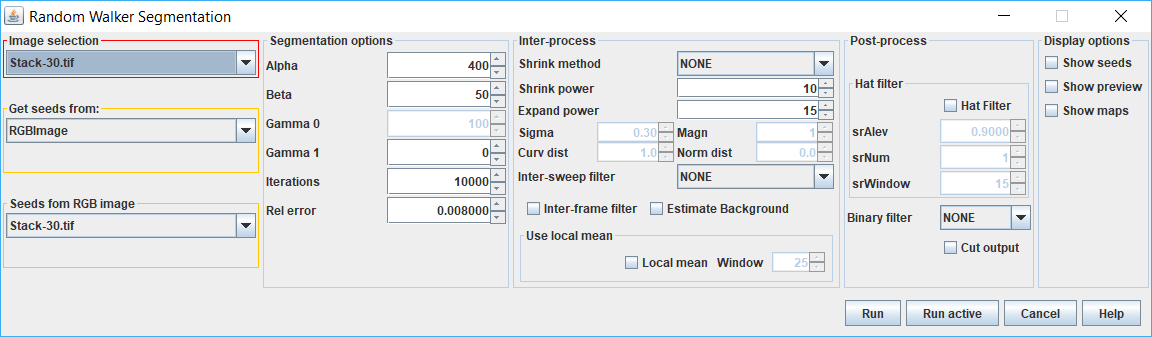
\includegraphics[width=18cm]{RandomWalkWindow.png} 
	\caption{Random Walker segmentation dialog}
	\label{fig:rwdialog}
\end{figure}

\textbf{Image section} - here user can select image that will be segmented. It must be grayscale image either 8 or 16 bits.

\textbf{Seeds section} - defines source of the seed image. The following options are available:
\begin{itemize}
	\item RGB image - user can provide RGB image where foreground pixels are labeled with pure red colour and background with pure green. The z-dimension of the seed image must equal to one or to the number of slices of segmented image. If there is only one slice of the seed given, it will be applied to the first slice of segmented image. For the \textit{n}+1 slice the seed will be generated using results of segmentation of \textit{n}-th slice processed by algorithm selected in \textit{Inter-processing section}.
	In this mode only one foreground object is supported.
	\item Create image - user can create RGB image cloned from the image selected in \textit{Image section} (\textit{Clone} button). The \textit{FG} and \textit{BG} buttons select foreground and background pen respectively.
	\item Mask image - user can provide grayscale image, where pixels of values grater than 0 stand for the foreground seeds. This mode is intended for using results of Active Contour segmentation as input to Random Walk algorithm. The seed stack should have the same size as segmented image. The foreground labels can be larger than objects they label because they are pre-processed (usually shrank) by algorithm selected in \textit{Inter-processing section}. Typical use case is to perform rough segmentation in BOA module using fail safe parameters which usually lead to rough segmentation and then to use Random Walk plugin to get fine one. The improvements should clearly visible especially in concave areas where Active Contour method fails. \textbf{Note} - providing mask as initial seed usually requires any \textit{Shrink method} to be set.      
	\item QCONF file - the same as \textit{Mask image} but user can provide \textit{QCONF} file saved in BOA module. Cells stored in the file are rendered to grayscale image, each cell is segmented independently from others.
	\item ROIs - initial seeds can be provided as ROIs. This mode also supports multi-object segmentation. There is simple tool available for collecting ROIs, described in \autoref{sec:CollectingROIs}.   
\end{itemize}
  
\textbf{Dynamic section} - its content depends on selected seed source.

\textbf{Segmentation options} - controls segmentation process. Options available here:
\begin{itemize}
	\item \textit{Alpha} - penalises pixels whose intensities are far away from the mean seed intensity
	\item \textit{Beta} - penalises pixels located at an edge, i.e. where there is a large gradient in intensity. Diffusion will be reduced.
	\item \textit{Gamma 0} - currently disabled
	\item \textit{Gamma 1} - set to 0 to skip second sweep. Other values are currently ignored.
	\item \textit{Iterations} - number of iterations (half of this number for second sweep)
	\item \textit{Rell error} - Relative error - stopping criterion for iterative Random Walk algorithm 
\end{itemize}

\textbf{Inter-processing section} - it controls how binary masks should be transformed to seeds internally. This process applies when seeds are given as result\textbf{Seeds section}s of segmentation from other method (\textit{Mask image} or \textit{QCONF file}) or there is only one slice of seeds provided (\textit{RGB image}). Binary mask is shrunk by algorithm selected in \textbf{Shrink method} with \textbf{Shrink power}. Results define object's seeds for next frame. Then, the same mask (unmodified) is expanded by the same algorithm but with \textbf{Expand power} and then inverted to define background seeds for the next frame. Options available here are:
\begin{itemize}
	\item Shrink method:
	\begin{itemize}
		\item \textit{NONE} - no shrinking or expanding. Mask is used directly as seed
		\item \textit{CONTOUR} - the ANA contour processing algorithm is used for modifying masks. They are first outlined then vectorised and finally processed. This approach preserves shape of the contour. Parameters \textit{Shrink power} and \textit{Expand power} relate to number of pixels to shrink and expand the contour respectively. Shrink power can be additionally function of local curvature, which is controlled by the following options:
		\begin{itemize}
			\item \textit{sigma} - sigma of Gaussian function used for computing \textit{Shrink power} multiplier for negative curvature. For positive curvature multiplier is explicitly set to 1.0. 
			\item \textit{Magn} - maximal value of multiplier. The Gaussian curve is scaled to give value of 1.0 around curvature of 0 deg and \textit{Magn} for large negative curvatures. Its slope depends on \textit{sigma}. Set it to 1.0 to get curvature independent scaling.
			\item \textit{Curv dist} - approximate number of nodes used for local averaging of curvature along outline. Values less than 3 usually give average over three nodes (current one, next and previous).
			\item \textit{Norm dist} - approximate number of nodes used for normales equalization. The algorithm looks for node with minimal curvature within this range and then set normales for all nodes in processed window to be same as in this node. Refer to \autoref{fig:shrinkcomp} for examples of \textit{Curv dist} and \textit{Norm dist} parameters.  
		\end{itemize}
		Generally, non-linear shrinking try to maintain shape of original contour but constricting it more around concave regions of the outline, that should reduce accidental miss-labeling the background.  
		\begin{figure}[ht]
			\centering
			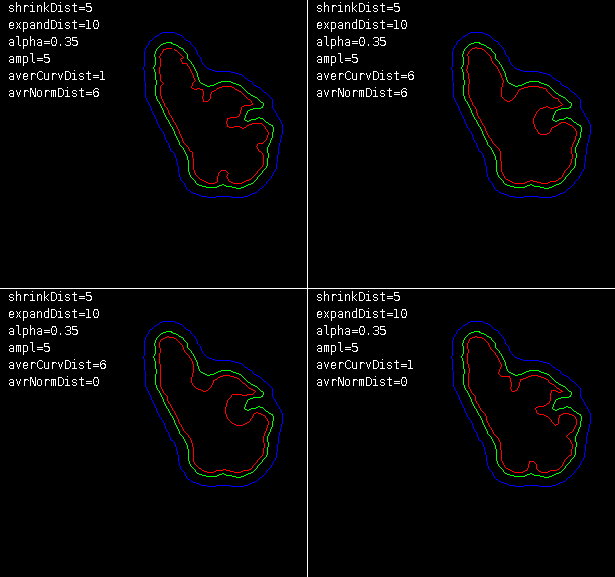
\includegraphics[width=14cm]{PropagateSeeds_Contour.png} 
			\caption{Nonlinear contour shrinking. Examples of different settings. Green - original contour, red - constricted contour, blue - expanded contour.}
			\label{fig:shrinkcomp}
		\end{figure}
		\item \textit{MORPHOLOGICAL} - masks are processed by morphological erosion. Parameters \textit{Shrink power} and \textit{Expand power} relate to number of algorithm iterations. 
	\end{itemize}
	\item Inter-sweep filter - applied between sweeps. It is intended to remove binary noise, isolated pixels, etc, that could give false seeding:
	\begin{itemize}
		\item \textit{NONE} - filtering disabled
		\item \textit{SIMPLE} - performs one iteration of morphological opening operation.
		\item \textit{MEDIAN} - median filtering with kernel of radius 2.
	\end{itemize}
	\item \textit{Estimate Background} - try to apply simple Otsu thresholding to background seeds. Use \textit{Show seeds} to verify correctness of estimation.
	\item \textit{Inter-frame filter} - apply additional erosion and median filtering between frames during propagation of seeds.
\end{itemize}

\textbf{Local mean} - this option can improve behavior of the algorithm in areas with high gradient of intensity, usually at cell cortex, preserving cell boundaries. This method works only with seeds provided as \textit{Mask image} or \textit{QCONF file}. Moreover, masks should be larger than the object itself. \textit{Window} parameter stands for the size (odd) of the sampling window used for computing local mean intensity.   

\textbf{Post-processing section} - it covers filtering of results applied after segmentation. The options are:
\begin{itemize}
	\item Hat filter - it tries to remove small inclusions in contour that typically came from vesicles located near cell edge. The algorithm is described \href{https://pilip.lnx.warwick.ac.uk/site/apidocs/index.html}{here}.
	\begin{itemize}
		\item \textit{srAlev} - acceptance level beyond the inclusion is removed
		\item \textit{srNum} - number of inclusions to remove. All they must have rank above \textit{srAlev}. If this parameter is set to 0, any inclusion with rank above \textit{srAlev} will be removed. 
		\item \textit{srWindow} - size of the processing window in pixels. Smaller window is more sensitive to small inclusions. 
	\end{itemize} 
	\item Binary filter - stands for the final filtering, the same algorithm are used as in \textit{Inter-processing section}.
	\item Cut output - output mask will be cut by input mask. This option assures that resulting mask is not larger than the seed mask.
\end{itemize}

\textbf{Display options section} - allows to show real time preview of each segmented frame and seeds computed as results of \textit{Iter-processing} binary masks. This option can be used for verifying \textit{Shrink power} and \textit{Expand power} settings. \textit{Show maps} display raw unscalled probability maps for each seed. This option does not work with stacks, only probability maps for last segmented frame are displayed.  

\subsubsection{Multi cell segmentation - Collecting ROIs}
\label{sec:CollectingROIs}
ROI collector is available after selecting \textit{ROIs} in \textbf{Seeds section}. This tool uses ImageJ ROI Manager to store ROIs that denote foreground and background seeds. The ROIs need to obey certain naming criterion, such as \textit{[LB][Id]\_[No]}, where \textit{LB} can be either \textit{fg} or \textit{bg} denoting foreground or background seed respectively, \textit{Id} is unique number of foreground object (only one or none background seeds are allowed) and \textit{No} is a sequence number of ROI for object of specified \textit{Id} (a seed for one object can be specified by several separate ROIs). 

The ROI collector tool (\autoref{fig:RoiTool}) manages proper naming of ROIs in the ROI Manager. After launching, the ROI Manager will be opened and its content erased. 

\begin{figure}[ht]
	\centering
	
\includegraphics[width=6cm]{RoiTool.png} 
	\caption{ROI collector tool used for selecting foreground and background objects.}
	\label{fig:RoiTool}
\end{figure}

User can label an image using standard ImageJ ROI objects and then click \textit{New FG} or \textit{new BG} to add current selection to ROI Manager. Each next use of \textit{New FG} will add new foreground object. If certain object ought to be labeled by separated ROIs, they should be added to ROI manager first (by \textit{Add} button) and then \textit{New FG} should be clicked. All ROIS in ROI Manager that do not follow specified naming convention are renamed and assigned to \textbf{one} object by \textit{New *} buttons. To finish labeling and transfer ROIs to the plugin click \textit{Finish} button.

\subsubsection{Random Walker Segmentation Workflow}
%TODO Add exampample of fine processing
If segmentation ends too early (e.g. result is very similar to seeds) one can open Fiji Console (\textit{Window}$\rightarrow$\textit{Console}) and check reason of stopping and relative error. If process stops due to reaching relative error in the first few iterations, one can adjust \textit{Rel error} accordingly.   

\subsection{Mask generator}
\label{sec:MaskGenerator}
This plugin can convert cells contours into binary image mask. The cell shape is represented by white area being a filled cell contour whereas the background in black. Masks are widely used in computer graphics for selecting regions of image for processing and analysing. ImageJ is also equipped with relevant procedures that allow for explicit processing masked regions. Therefore, this plugin make it possible to continue analysis of the sample outside the QuimP infrastructure.

Mask Generator plugin works with \textit{QCONF} files saved by BOA module. It is not possible to use it with old file format (paQP) unless it has been converted to \textit{QCONF} by Format Converter (available from QuimP Toolbar menu). By default, the mask image is displayed on the screen and saved on disk at location of input \textit{QCONF} file with suffix \textit{snakemask}.

This plugin supports ImageJ macro language. Use \textit{Macro Recorder} to discover the syntax.

\subsubsection{Suggested workflow}

\begin{itemize}
	\item Run Mask Generator plugin from QuimP toolbar (\autoref{fig:quimpBar}).
	\item Point to \textit{QCONF} file to process. This plugin does not support old \textit{paQP} files (but they can be converted to ne file format by Format Converter, refer to \autoref{sec:DataFilesExplained}).
	\item Binary mask image, converted from contours stored in QCONF file by BOA module will be displayed on the screen and saved on disk (Fig. 3). Default saving location is the location of opened QCONF file. The quality of mask depends on the quality of segmentation and the number of nodes configured in BOA module.
	\item Use \texttt{Edit$\rightarrow$Selection$\rightarrow$Create Selection} to convert binary mask to ImageJ ROIs. Then, it can be populated through ROI manager to e.g. source image.
\end{itemize}

\section{Protrusion tracking}
\label{sec:ProtTracking}

Protrusion Analysis module allows investigating protrusion formation and dynamics.

Protrusions are detected by finding local maxima in the motility map. After decoding from the motility map coordinates (\textit{outline index}, \textit{frame}) to Cartesian coordinates (\textit{x}, \textit{y}, \textit{time}), those points are considered as origins of the protrusions. Every origin point can be tracked backward and forward in time as long as its velocity is above certain level, related to the velocity of origin point.

The module requires \textit{QCONF} file that contains full description of QuimP analysis. Particularly, the BOA, ECMM an Q Analysis modules should be run on \textit{QCONF} before using Protrusion Analysis.

The user interface is shown below.

\begin{figure}[ht]
	\centering
	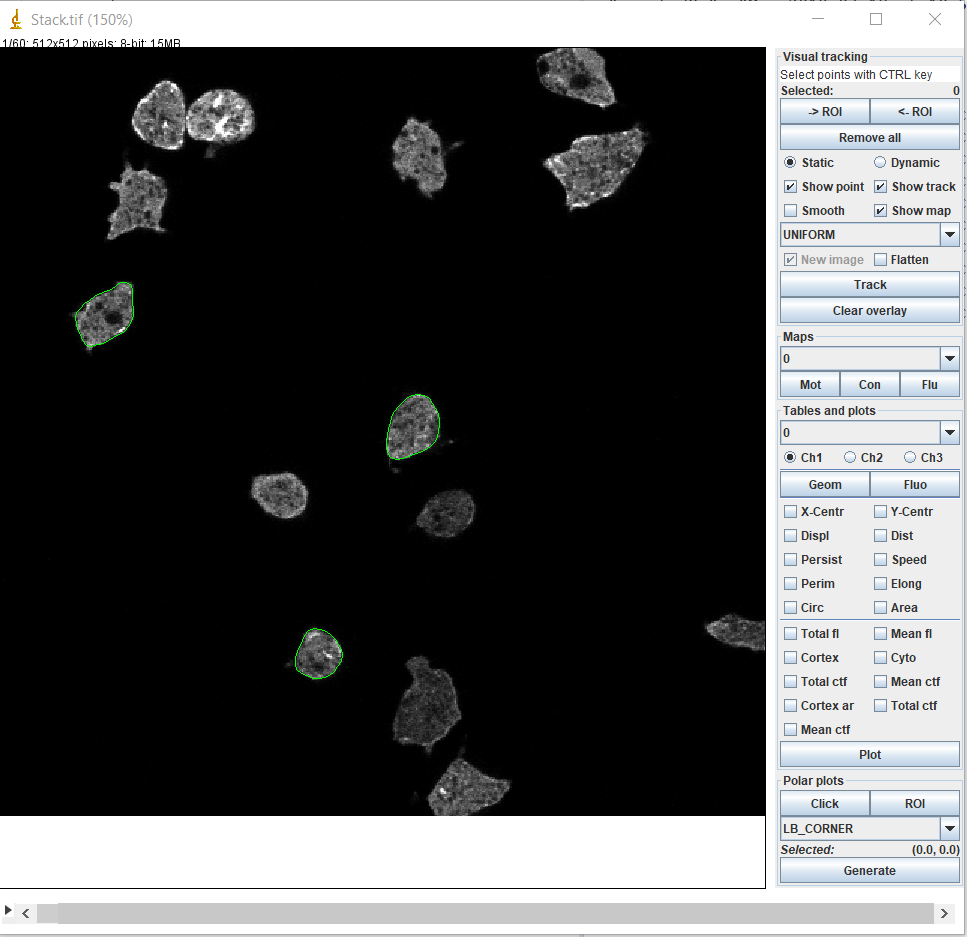
\includegraphics[width=16cm]{protrusion_window.png} 
	\caption{Protrusion Analysis module dialog}
	\label{fig:protrusiondialog}
\end{figure}

\begin{itemize}
	\item Options section - contains mandatory settings for peaks detection.
	\begin{itemize}
		\item \textit{Drop} - defines how long the origin point $p(t0)$ from time frame $t0$ should be tracked forward and backward in term of the change of its velocity in time. The point for time frame $t$, $p(t)$ is tracked as long as its velocity $v_{p(t)}$ meets the criterion $v_{p(t)}>v_{p(t0)}*(1-Drop)$.
		\item Sens - Peak detection sensitivity. The module uses standard ImageJ \texttt{Process$\rightarrow$Find Maxima} algorithm.
	\end{itemize} 
	\item Info section - shows basic information about found number of peaks, data range and gradient position.
	\item Map plots - allows to select what map plots are produced after analysis. The \textit{Maxima} map contains also peaks points and tracks.  
	\item Outline plots section - allows to plot cell outlines colored according to chosen algorithm. E.g. selecting \textit{Plot type}$\rightarrow$\textit{MOTILITY} and \textit{Mot Thr}=\textit{0}, one will get colored only those parts of outline that have velocity above 0.
	\item Maxima plot section - contains different methods of data visualization.
	\item Dynamic plot section - allows to produce image stacks with peaks and tracks changing in time.
	\item Polar plot section - saves on disk polar plot. Polar plot represents local velocity of the cell membrane averaged over time for each node (owing ECMM algorithm, the cell contour can be interpolated to any real number of nodes that can be tracked forward and backward in time). Point on the contour that is closest to location of chemotactic gradient source is considered as the first one at polar coordinate $\theta=0^{\circ}$.
\end{itemize}
  
Every time when \textit{Apply} button is used, the module runs new analysis and produces all plots selected in relevant sections.  

\section{Data Files Explained}
\label{sec:DataFilesExplained}

\subsection{Parameter files - new format vs. old format}
The latest QuimP introduces a new file format called QCONF\footnote{above QuimP11}. The \textit{QCONF} is based on human-readable JSON format and it is designed to hold all results evaluated by QuimP on every stage of data processing, together with configuration parameters, algorithm settings, etc. 
Initially, the \textit{QCONF} is generated by BOA plugin together with \textit{stQP} file (the same statistical measurements are also contained in \textit{QCONF}, \textit{stQP} file is saved separately for convenience sake). Remaining modules depend on \textit{QCONF}, thus they read and write all data from/to this file. The \textit{QCONF} is not replacement for "old" formats - it rather extends them and allows for easy sharing of results between different QuimP modules, restoring work from last point and keeping the whole QuimP configuration in one place.   

Currently, QuimP understands both formats, but its behavior depends on the status of tick box available in QuimP Toolbar (\autoref{fig:quimpBar}) and on format loaded to module:
\begin{itemize}
	\item \textit{Use new file format} is selected - only \textit{QCONF} files are shown in file chooser\footnote{This feature may not work correctly on Windows systems}. A \textit{QCONF} loaded to QuimP module will be updated and saved back. Files in previous format (\textit{paQP}, \textit{snQP}, \textit{maQP}, \textit{stQP.csv}) \textbf{are not} saved but they can be optionally regenerated by Format Converter\footnote{Available from QuimP Toolbar $\textit{Tools}\rightarrow\textit{Format Converter}$} in the same directory. \textbf{This is recommended approach.}
	\item \textit{Use new file format} is deselected - both configuration files (\textit{paQP} and \textit{QCONF}) are shown in file chooser. The \textit{paQP} files are generated every time, even if user loaded \textit{QCONF} file. The \textit{QCONF} file \textbf{is not} updated or generated if user loaded \textit{paQP}. 
\end{itemize}   

Relations between module and file are summarized in \autoref{filestable}. Legend for \autoref{filestable} is as follows:
\begin{itemize}
	\item \textbf{N} - file is created.
	\item \textbf{M} - file is modified - new data are appended to it.
	\item \textbf{C} - file is changed - some data are replaced.
\end{itemize}

\textbf{Note} \\
The \textit{QCONF} file can be loaded to Matlab using one of the free JSON parsers (tested with JSONlab\footnote{\url{http://uk.mathworks.com/matlabcentral/fileexchange/33381-jsonlab--a-toolbox-to-encode-decode-json-files}}).

\begin{table}[h]
	\centering
	\caption{Relation among modules and generated files}
	\label{filestable}
	\begin{tabular}{|l|l|l|l|l|l|l|l|l|}
		&  \textbf{paQP}&  \textbf{snQP}&  \textbf{maQP}&  \textbf{stQP.csv}&  \textbf{QCONF}&  \textbf{pgQP}& \textbf{svg}&  \textbf{tiff}\\ \hline
		\textbf{BOA} &   N&  N&  &  N&  N&  N&  &  \\
		\textbf{ECMM}&    &  C&  &   &  M&   &  &  \\
		\textbf{ANA} &   M&  M&  &  M&  M&   &  &  \\
		\textbf{Q Analysis}&  &  &  N&  &  M&  &  N& N 
	\end{tabular}
\end{table}


\subsubsection{Conversion between formats}
\label{sec:ConversionBetweenFormats}
QuimP supports conversion between old \textit{paQP} and new \textit{QCONF} formats. Simple tool for this purpose is available from the QuimP bar (see \autoref{fig:quimpBar}) under \textit{Tools} menu or in extended version as separate module (see \autoref{fig:formatconverter}). The module additionally allows to extract numeric data from \textit{QCONF} and save them in user friendly \textit{csv} format.

\begin{figure}[h]
	\centering
	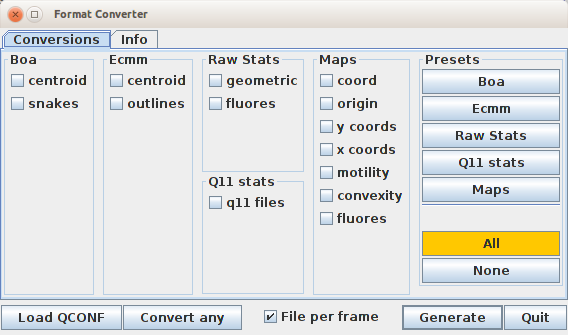
\includegraphics[width=16cm]{fcWindow.png} 
	\caption{Format converter dialog.}
	\label{fig:formatconverter}
\end{figure}

\textbf{Conversion between formats - \textit{Convert any} button}

Conversion tool is available from either the QuimP bar or Format Converter module under \textit{Convert any} button. After selecting proper input file - \textit{QCONF} or \textit{paQP}, the opposite format is saved in the same folder. The following rules will apply:
\begin{enumerate}
	\item If \textit{paQP} is an input file, it must be the first one with suffix \textit{\_0.paQP}.
	\item The \textit{QCONF} format stores separate segmentation settings for each frame - only settings from the first frame are saved in \textit{paQP}. 
	\item Order of outline nodes in \textit{QCONF} can be randomly shifted forward or backward by one node during conversion from \textit{paQP}. 
	\item \textit{paQP} format stores data with precision limited to two decimal places.
\end{enumerate}

\textbf{Extracting data from \textit{QCONF} format - \textit{Load QCONF} button}

Format converter module (\autoref{fig:formatconverter}) allows to save selected parameters evaluated during QuimP workflow and stored in \textit{QCONF} file as separate \textit{csv} files. Some parameters (like e.g. those under \textit{Raw Stats}) coincide with content of \textit{snQP} or \textit{stQP.csv} files. Data extraction is applicable only to \textit{QCONF} files that should be loaded by \textit{Load QCONF} button. Conversion process is initiated by \textit{Generate} button. Output files are saved in the same folder as input \textit{QCONF}.    
  
\subsection{Parameter Files - \textit{paQP} Files}
\label{paQP}

A parameter file contains text and has the extension \textit{.paQP}.  Both QuimP's plugins and
Matlab functions use the parameter file to locate files associated with an analysis and also to store data such as the
pixel size, frame interval, and start frame.  In addition, it stores the parameters used for segmentation
(the last used parameters).

The first line identifies the file as a QuimP parameter file, and contains the creation date.
The second is random identifier.
The third is the absolute path to the image used for segmentation.
 
In general, the contents of a parameter file should not be changed, but you may wish to alter the paths to
image files if you later move them.
 

\subsection{Snake Data - snQP files}
\label{snQP}

The \textit{.snQP} file contains data relating to the nodes of cell outlines (\textit{snake} is a reference to active contours being 
described as snakes).   Comment lines
begin with a \#.  Data for frame $f$ begins with the comment line \textit{\#frame f}, followed by a single integer value
indicating the number of nodes that make up the outline ($N$).  The following $N$ rows hold the data for the nodes. The 
columns are as follows:

\begin{itemize}

\item \textbf{Node Position} - The normalised position of the node in relation
to node zero, $n_{0}$ (see \autoref{ecmmTracking}).

\item \textbf{X\_coord} - The horizontal pixel coordinate of a node on the image used for segmentation.

\item  \textbf{Y\_coord} - The vertical pixel coordinate of a node on the image used for segmentation.

\item \textbf{Origin} - The position from which a node originated from on the outline
at the previous frame (see \autoref{ecmmTracking}).

\item \textbf{Global Origin} - The position from which a node originated from on the outline
at the first segmented frame (see \autoref{ecmmTracking}).

\item \textbf{Speed} [microns per second]- The speed at which a node travelled between frames, as determined by ECMM.

\item \textbf{Fluor\_Ch\$} - The intensity value assigned to a node by ANA (see \autoref{ana}) for the channel
number denoted by \$.  This value is the maximal $3x3$ average intensity measured at the node's local cortical region.

\item \textbf{Ch\$\_x} - The horizontal pixel co-ordinate on the fluorescence image at the point where Fluor\_Ch\$ was measured, i.e.
the co-ordinate where the maximum intensity occurred.

\item \textbf{Ch\$\_y} - The vertical pixel co-ordinate on the fluorescence image at the point where Fluor\_Ch\$ was measured, i.e.
the co-ordinate where the maximum intensity occurred.

It is possible to store data for 3 fluorescence channels ($\$=\{1,2,3\}$) within the \textit{.snQP} file. Missing 
data is denoted by negative values.

\end{itemize}

\subsection{Frame statistics - stQP files}
\label{stats}

The statistics file, with the extension \textit{.stQP}, contains whole cell statistics for each frame (rather than node associated
data).  Data is written as \textit{comma separated values} which can be opened easily as a spreadsheet.  The file is split into
two section.  Data in the top section is computed by BOA and relates to cell morphology and movement of the cell centroid.
Data in the lower section relates to cell fluorescence and was computed
by ANA (data is listed separately for all 3 available channels). Missing data is denoted by $-1$.

The cell centroid is computed as the weighted centre of the polygon formed by the cell outline.
The measures computed by BOA are as follows:

This file is generated and updated regardless of selected file format (\textit{QCONF} or \textit{paQP}). Refer to \autoref{filestable}
 
\begin{itemize}

	\item \textbf{X-Centroid} [$pixels$] - Horizontal pixel co-ordinate of the cell centroid.

	\item \textbf{Y-Centroid} [$pixels$] - Vertical pixel co-ordinate of the cell centroid.
	
	\item \textbf{Displacement} [$microns$] - Distance the cell centroid has moved from its position in the first recorded frame. 
	
	\item \textbf{Distance Travelled} [$microns$] - Sum of the centroid displacements between frame, i.e. the total distance 
	over which the centroid has moved.
	
	\item \textbf{Directionality} - Persistence in direction, calculated as $Displacement / Dist. Travelled$ (chemotaxis index). A value of 1 reveals that
	a cell has moved in a straight line.  Decreasing values denote a cell moving increasingly erratically.
	
	\item \textbf{Speed} [$microns~per~second$] - Speed at which the centroid moved between the current and previous frame.
	
	 \item \textbf{Perimeter} [$microns$] - Length of the cell perimeter (segmented outline).
	  
	 \item \textbf{Elongation} - An ellipse is fitted to the cell outline and the major/minor axis used to compute the elongation of 
	 the cell's shape. $Elongation = major~axis / minor~axis$. Note that a value of 1 does not necessarily represent
	 a perfectly circular cell, only a circular fitted ellipse.
	 
	 \item \textbf{Circularity}  - A measure of circularity defined by the following equation:
	$\frac{4*PI*Area}{Perimeter^{2}}$. A value of 1 reveals the cell's outline to be perfectly circular.
	 
	 \item \textbf{Area} [$microns^{2}$] - Cell area.
	 
\end{itemize}

The measures computed by ANA are as follows:

\begin{itemize}

	\item \textbf{Total fluo.} [$pixel intensity$] - Total fluorescence. Sum of all pixel intensities within the cell outline. 

	\item \textbf{Mean fluo.} [$pixels intensity$] -  Mean fluorescence. Average intensity of pixels within the cell outline.

	\item \textbf{Cortex width} [$microns$] - Width of the cortex, as specified by the user (see \autoref{ana}).
	
	\item \textbf{Cyto. area} [$microns^{2}$] - Area of the cytoplasm (area of the whole cell minus the cortex area).
	
	\item \textbf{Total cyto. fluo.} [$pixels~intensity$] - Sum of all pixel intensities within the cytoplasm. 
	
	\item \textbf{Mean cyto. fluo.} [$pixels~intensity$] - Average pixel intensity within the cytoplasm.
	
	\item \textbf{Cortex area} [$microns^{2}$] - Area of the cortex.
	
	\item \textbf{Total cortex fluo.} [$pixels~intensity$] - Sum of all pixel intensities within the cortex. 
	
	\item \textbf{Mean cortex fluo.} [$pixels~intensity$] - Average pixel intensity within the cortex.
	
\end{itemize}


\subsection{QuimP Maps - maQP files}
\label{maps}

The images produced by Q Analysis are spatial-temporal maps of motility, convexity, and fluorescence.  The vertical axis represents 
time, with frame 1 at the top.  The horizontal axis represents positions along the cell outline, the length of which
has been normalised to 1 at every frame.  Outlines can be
thought of as having been `cut' at position zero, laid along the horizontal axis, and stacked below one another, hence maps
are cylindrical (wrap around onto themselves on the horizontal axis). 

The node randomly designated as begin node zero ($n^0$), at frame 1, is mapped to the top left
pixel.  Data from ECMM is used to track the position of $n^0$
throughout all the frames, and is always positioned at the left most pixel at each frame.  All other nodes are positioned along 
the horizontal axis according to their distance from $n^0$ 
along the cell perimeter.  Values between nodes are estimated using linear interpolation. 

If the number of frames is below the specified map resolution, then maps are scaled vertically, hence 
a row of pixels may be an interpolated value between frames.  

As well as producing \textit{.tif} images, maps are also 
saved as text images with the extension \textit{.maPQ}.  Unlike the \textit{.tif} maps, these are not scaled vertically, so each line of 
values contains the data for a single frame.  It is these maps that should be used for further analysis.

Similarly, four additional maps are produced to aid further analysis:

\begin{itemize}

\item \textbf{Motility Map.}   Pixels are coloured according to node speed, as calculated by ECMM.  Red shades 
represent expanding regions, blue shades contracting regions.  Pixel values
within the \textit{tiff} image are scaled to fill the colour spectrum.  The map file extended \textit{\_motilityMap.maPQ} contains 
un-scaled values, in \textit{microns per second}. 

\item \textbf{Fluorescence Maps}.  A fluorescence map is produced for each channel that data has been 
recorded into.  The fluorescence map images display pixel intensities, as extracted by the ANA plugin.
Files extended \textit{\_fluoCh\$.maPQ} contain the respective data. Fluorescence value is a mean of pixel intensities sampled within 9-point stencil for each node of the cortex outline (see \autoref{ana}).

\item \textbf{Convexity Map}.   Represents the curvature of the cell, measured in the range $[-1,1)$, where negative values are concave (blue),
and positive convex (red).
As with the motility map, values
are scaled to fill the colour map. Files extended \textit{\_convexityMap.maPQ} contain the respective data (un-scaled). 

\item \textbf{Co-ordinate Map (a.k.a. Position Map)}.  As described in \autoref{ecmmTracking}, each node has an
associated position.  The co-ordinate map, rather than contain values regarding
motility, fluorescence or convexity, instead contains the position values of nodes.  The main
purpose of the co-ordinate map, along with the origin map, is for tracking positions through time (see \autoref{trackingMaps}).

\item \textbf{Origin Map}. As described in \autoref{ecmmTracking}, each node has an origin, the position a node originated from
on the previous frame.  The origin map contains origin values and can be used, along
with the co-ordinate map, to track positions through time (see \autoref{trackingMaps}).

\item \textbf{xMap}.  Contains horizontal image pixel co-ordinates (those on the image used for segmentation) relating to map pixels.

\item \textbf{yMap}.  Contains vertical image pixel co-ordinates (those on the image used for segmentation) relating to map pixels.

\end{itemize}


\subsection{Scalable vector graphics output - svg files}

Files extended with
\textit{.svg} can be viewed natively in most internet browsers (Windows Explorer requires the Adobe SVG viewer), or opened and edited
in graphics software ( e.g. Inkscape, free software for mac).  The 
Scalable Vector Graphics (svg) file format can be viewed at any desired resolution. 

\begin{itemize}

\item \textbf{Cell track}.  An overlay of all cell outlines coloured according to frame number. Files extension \textit{\_track.svg}.

\item \textbf{Cell motility movie}.  Data contained within the motility/fluorescence/convexity map is displayed on the cell track. Extension \textit{\_motility.svg}.

\end{itemize}

\subsection{BOA plugins stack configuration - pgQP file}

This file stores configuration of plugin stack together with configurations of active plugins (see \autoref{boaWindow} and \autoref{sec:boaFilters}). This file is not related to any loaded data therefore it can be exchanged between projects. Complex plugin stack configuration is stored also in \textit{QCONF} file. 

%\section{Tracing paths through frames}

%This section will describes methods for tracking positions through time. See \autoref{trackingMaps}.

\section{ImageJ macro support}
\label{sec:macrosupport}
Most of QuimP modules support ImageJ macro language but syntax of the command (especially parameters passed to the module) differs from that commonly used by other ImageJ plugins. Use Macro Recorder tool to discover parameters supported by plugin. Note that any file name or path should be enclosed in parentheses if it contains spaces. Windows users should use slash symbol in path names (e.g. c:/Users/myfile.QCONF). Quote character is not allowed in parameter string. Skipped parameters get their default values, therefore output from Macro Recorder can be greatly reduced by removing options that are not used or unchanged. 

Note that macro strings are outputed to Macro Recorder only if plugin is run from Menu. \textbf{It does not work if plugin has been started from QuimP Toolbar.}
 
\section{MATLAB Functions}
\label{matlab}

Archive with Matlab routines mentioned in this section is available on \href{http://www2.warwick.ac.uk/fac/sci/dcs/people/till_bretschneider/quimp/test_data}{QuimP web page (section Download QuimP)}\footnote{http://www2.warwick.ac.uk/fac/sci/dcs/people/till\_bretschneider/quimp/test\_data}

\noindent\fcolorbox{red}{yellow}{
	\parbox{\textwidth} {
		Matlab routines work with old data format only (\textit{*.paQP}, \textit{*.snQP}, etc.). To use them with \textit{QCONF} file, it has to be first converted to the old format by Format Converter (\autoref{sec:DataFilesExplained}). It is also possible to load \textit{QCONF} to Matlab using JSon readers.  
	}
}

QuimP outputs a large amount of data for each cell analysed.
You may want to write custom scripts for analysis, but we provide
a set of MATLAB functions to remove the hassle of loading/organising data, and performing
simple operations, such as plotting maps.
We hope to make data as accessible and as explorable as possible to allow adaptation to a users specific goals.

Help documentation is included with each function which can be accessed in the
usual way by typing \textit{help functionName} at
the MATLAB command prompt.  At the end of this document is a walkthrough analysis using the provided test images
(see \autoref{walkthrough}).

\subsection{Loading data - \textit{readQanalysis.m}  }

The first step is to launch the script \textit{readQanalysis.m} which handles loading of data from multiple
cells.  Given a directory, it will search that directory, and all sub-directories, for \textit{.paQP} files. For each parameter file
that is found an analysis structure is built.  As data is read from sub-directories, you may organise your separate analyses into 
sub-directories, but placing all files into the same directory is still possible. Missing files are skipped, hence it is not necessary to have run all the QuimP plugins.


Loading data relies on the maintenance
of file names imposed by the QuimP plugins, and requires associated files to
be present in the same directory as the parameter file.
The exceptions to this are the images used for segmentation and fluorescence measurements.  Paths to these images are
stored in full to allow separation of analysis files from image data.  If images are moved, and subsequently cannot
be located, the directory where the parameter file is stored will be searched.  You may edit the \textit{.paQP} file to alter
paths to the images if you wish
(note that images are not loaded into memory by \textit{readQanalysis.m}, instead the function checks only that they exist
and sets a path to them).

The output of \textit{readQanalysis.m} is an array of structures, $C$, each element holding data for a single analysed cell.
The contents of an analysis structure is as follows ($F$ = number of frames, $N^{f}$ = number of nodes at frame $f$):

\begin{itemize}

 \item \textbf{name} [$string$] - File name element common to all associated files (name of the parameter file).
 
  \item \textbf{index} [$integer$] - Cell ID, in order read in.
 
 \item \textbf{PATH} [$string$] - Directory of the parameter file.
 
 \item \textbf{\$FILE} [$string$] - Filenames of  QuimP output.
 
 \item \textbf{\$TIFF} [$string$] - Filenames of an image sequences.
 
  \item \textbf{outlines} [$cell~array~(F\times1)$]  - Holds node associated data. Each element
 contains a matrix of size $N^{f}\times6$,
each row being a node. Column headers are [Position , X-coord , Y-coord , Origin , Global origin ,  Speed].
 
 \item \textbf{outlineHeaders} [$cell~array~(1\times6)$] - Descriptions of column measures within \textit{outlines},
  as stated above.
  
 \item \textbf{fluo} [$cell~array~(F\times1)$] - Holds node fluorescence data for all three channels. Each element contains a 
  3D matrix of size $N^{f}\times3\times3$.  The first dimension represents nodes, second the channel number, and third the
  measure.   The measures are [Intensity , X-coord , Y-coord], where the x and y co-ordinates provide the location of
  sampling (see \autoref{ana}).  For example, the intensity sampled at node 23, on channel 2 is located at (23,2,1).
  
 \item \textbf{fluoHeaders} [$cell~array~(1\times3)$] - Descriptions of measures within \textit{fluo}, as 
 stated above.
 
 \item \textbf{nbFrames} [$integer$] - The number of frames.

 \item \textbf{startFrame} [$integer$] - The first frame segmented relative to the the image used for segmentation.

 \item \textbf{endFrame} [$integer$] - The last frame segmented relative to the the image used for segmentation.

 \item \textbf{frames} [$vector~(F\times1)$] - Vector of the segmented frames relative to the the image used for segmentation.
 
  \item \textbf{PixelSize} [$double$] - Pixel size in microns (image scale).

 \item \textbf{frameInterval} [$double$] - Frame interval in seconds.
  
 \item \textbf{R} [$vector~(1\times4)$] - Pixel co-ordinates of a bounding box encompassing all movement of the cell.
 R = [x min, x max, y min, y max]. 
 
  \item \textbf{maxSpeed} [$vector~(F\times1)$] - For each frame the maximum node speed is calculated.
  This is useful for scaling plots.

 \item \textbf{stats} [$matrix~(F\times11)$] - Holds whole cell statistics relating to the cell centroid and cell shape (see
 \autoref{stats}).  Rows contain data for frames.  The column headers are ['Frame'    'x-Centroid'    'Y-Centroid' 
 'Displacement'   'Distance Travelled'    'Directionality'  'Speed'    'Perimeter'    'Elongation'    'Circularity'    'Area']

  \item \textbf{statsHeaders} [$cell~array~(1\times11)$] - Descriptions of column measure within \textit{stats}, as stated above.
  
  \item \textbf{fluoStats} [$matrix~(F\times3\times11)$] - Holds global cell statistics relating to the cell fluorescence (as described in
 \autoref{stats}).  The first dimension is frame number,  second the channel number, and third the measure.  The 
 measure headers are ['Frame'    'Total Fluo.'    'Mean Fluo.'    'Cortex Width'    'Cyto. Area'    'Total Cyto. Fluo.'
  'Mean Cyto. Fluo.'    'Cortex Area'    'Total Cortex Fluo.'    'Mean Cortex Fluo.'    '\%age Cortex Fluo.'].  Missing data is represented
  by negative values, typically $-1$.
  
  \item \textbf{fluoStatHeaders} [$cell~array~(1\times3)$] - Descriptions of the measures in the third dimensional
  within \textit{fluo}, as stated above.
  
  \item \textbf{cortexWidth} [$vector~(3\times1)$] - Holds for each channel the cortex width specified when running ANA. 
  
   \item \textbf{$\ast$Map} [$matrix~(F\times MapRes)$] - Maps read from \textit{.maQP} files (see \autoref{maps}).  A QuimP map 
   in MATLAB is a 2D matrix, rows being frames, columns being discrete points along the cell outline.

  \item \textbf{forwardMap} - see \autoref{trackingMaps}.
  
  \item \textbf{backwardMap} - see \autoref{trackingMaps}.
     
\end{itemize}


\subsection{Function Overview}

Functions prefixed with `read'  are used by \textit{readQanalysis.m} and so generally are not used
independently, but can be if desired.    For details of usage please refer to the
functions help by typing \textit{help functionName} at the MATLAB command prompt.

\begin{itemize}

 \item \textbf{buildTrackMaps} - Constructs the \textit{forwardMap} and \textit{backwardMap} based 
 upon the co-ordinate and origin maps.  These are used to track through QuimP maps.  See \autoref{trackingMaps} for details.
 
 \item \textbf{mapLookup} - Extract values from maps by specifying a window or region.  This can be used, for example, to extract data
 along tracked paths.
 
 \item \textbf{plotMap} - Plot a QuimP map using specified colour map limits.
 
 \item \textbf{plotMotility} - Plots a cell outline with nodes coloured according to their speed of movement.
 
 \item \textbf{plotOutline} - Plots a cell outline.
 
 \item \textbf{trackBackwards} - Utilises the \textit{backwardMap} to track backwards through a map, from a specified point,
 in accordance with the ECMM tracking data. 
 
 \item \textbf{trackForwards} - Utilises the \textit{forwardMap} to track forwards through a map, from a specified point,
 in accordance with the ECMM tracking data.
 
  \item \textbf{trackForwAcc} - Similar to \textit{trackForwards} but functions at sub-pixel resolution. More accurate but slower.
   
 \item \textbf{xcorrQ} - Perform cross-correlation and auto-correlation of .maPQ maps.
 
 \end{itemize}

\subsection{Tracking Maps}
\label{trackingMaps}

The term \textit{tracking} in this sense refers to being able to pick a position on the perimeter of a cell and identify its corresponding
position in the following frames, and hence, track a position over time.  The trace of a position, computed by ECMM,
can be plotted on top of a QuimP map. 

A QuimP map in MATLAB is a 2D matrix, rows being frames ($f$) and columns being discrete locations along the cell outline ($l$).
An incorrect view may be that a map pixel $p$ at frame $f$, and location $l$, ($p^{f}_{l}$),  tracks to the pixel directly 
below ($p^{f+1}_{l}$).  This is not the case,
$p^{f+1}_{l}$ does not necessarily originate from $p^{f}_{l}$.  The origin map must be consulted to identify the
correct location.

[Maps that enforce $p^{f}_{l}$ tracking to $p^{f+1}_{l}$ become heavily distorted, and certain regions lose
resolution severely.]

To track from $p^{f}_{l}$ to $p^{f+1}_{l2}$ we require the correct matrix column index at $f+1$, $l2$.  Firstly, 
consult the co-ordinate map at $p^{f}_{l}$ to identify the position on the cell outline.  Next, extract
the values in row $f+1$ from the origin map.  The index $l2$ is simply the index of the closest origin value to $p^{f}_{l}$'s position
(this can also be done at sub-pixel resolution for more accuracy).
The process is repeated to find $p^{f+2}_{l3}$, $p^{f+3}_{l4}$, etc.  In a similar way, positions can be tracked backwards in time.

This tracking procedure is implemented in the provided MATLAB functions. The function \textit{buildTrackMaps.m} creates
two additional maps, \textit{forwardMap} and \textit{backwardMap}, and is called when data is read in.
An element in the \textit{forwardMap}, for example at $p^{f}_{l}$, contains the correct column index for $l2$ to
locate $p^{f+1}_{l2}$.  Similarly, \textit{backwardMap} contains the correct values for finding $p^{f-1}$.

Functions \textit{trackForwards.m}, \textit{trackForwAcc.m} and \textit{trackBackwards.m}, given a frame, location,
and number of frames to track over, will return complete traces for you.
Consult the help for these functions for details of usage and the walkthrough for an example.

\section {Historical versions}

\subsection{QuimP11b}

\begin{enumerate}
	\item Fixed several minor bugs.
	\item Updated and tested with ImageJ 1.49a and MATLAB 2014a
	\item The ECMM and Q Analysis plugins will search for other .paQP in a directory and prompt to batch process files.
	\item BOA prompts to check image scale.
	\item BOA can read in a previous segmentation using the LOAD button
	\item When editing segmentations the user can scroll between frames without leaving edit mode
\end{enumerate}

\section{Contact}

The QuimP software is being developed at the Department of Computer Science at the University Of Warwick by the Till Bretschneider group (\href{mailto:till.bretschneider@warwick.ac.uk}{Till.Bretschneider@warwick.ac.uk}).
Further information, and future releases, can be obtained from \url{http://go.warwick.ac.uk/quimp}.

QuimP is under continuous development and feedback will be much appreciated.  If you discover a bug, have suggestions 
for features, or simply find a spelling mistake, please contact the developer Piotr Baniukiewicz at \href{mailto:p.baniukiewicz@warwick.ac.uk}{p.baniukiewicz@warwick.ac.uk}. Thank you for supporting our software. 
\bibliographystyle{plain}
\bibliography{references} 
\end{document}


















